%\documentclass[12pt]{article}
\documentclass[9pt]{sigplanconf}
% The following \documentclass options may be useful:
%
% 10pt          To set in 10-point type instead of 9-point.
% 11pt          To set in 11-point type instead of 9-point.
% authoryear    To obtain author/year citation style instead of numeric.
%\usepackage{bera}\usepackage[T1]{fontenc}
\renewcommand{\ttdefault}{txtt}
\usepackage{alltt}
\usepackage{listings}
\lstset{language=ML,
basicstyle=\ttfamily\footnotesize,
morekeywords={newcase,extends}}
\usepackage[usenames,dvipsnames]{color}
\usepackage[usenames,dvipsnames]{xcolor}
\usepackage{mathpartir}
\usepackage{amsmath}
\usepackage{amssymb} 
\usepackage{amsthm}
\usepackage{ stmaryrd }
\usepackage{graphicx}

\usepackage[noindentafter]{titlesec}
%\titlespacing{\section}{0pt}{*0.5}{*0.25}
%\titlespacing{\subsection}{3pt}{*1.5}{*0.25}
%\titlespacing{\subsubsection}{3pt}{*1.5}{*0.25}
%\titlespacing{\paragraph}{0pt}{*0.5}{*1}
\usepackage{textpos}
\newcommand{\lamA}{\lambda_{\text{A}}}

\newcommand{\tvarCtx}{\Delta}
\newcommand{\fCtx}{\Sigma}
\newcommand{\itvarCtx}{\Omega}
\newcommand{\iCtx}{\Theta}
\newcommand{\eCtx}{\Gamma}
\newcommand{\etvarCtx}{\Omega}
\newcommand{\fSpec}[3]{\tof{\fvar{#1}}{\kFam{#2}{#3}}}
\newcommand{\fSpecStd}{\fSpec{fam}{\kappaidx}{\Theta}}

\newcommand{\errCtx}{\mathcal{E}}
\newcommand{\famEvalCtx}{\Xi}

% Generic stuff
\newcommand{\pipe}{~\text{\large $\vert$}~}
\newcommand{\splat}[3]{#1_{#2},\ldots,#1_{#3}}
\newcommand{\splatC}[3]{#1_{#2}~~~~\cdots~~~~#1_{#3}}
\newcommand{\splatTwo}[4]{#1_{#3}#2_{#3},~\ldots~, #1_{#4}#2_{#4}}
\newcommand{\substn}[2]{[#1]#2}

% \psi
\newcommand{\psiu}[1]{{\psi_{#1}}}
\newcommand{\psit}[1]{{\psi_{\text{#1}}}}
\newcommand{\psitype}{\psit{type}}
\newcommand{\psiproof}{\psit{proof}}
\newcommand{\psiidx}{\psit{idx}}
\newcommand{\psiidxn}[1]{\psit{idx,#1}}
\newcommand{\psirep}{\psit{rep}}
\newcommand{\psirepn}[1]{\psit{rep,#1}}
\newcommand{\psiden}{\psit{den}}
\newcommand{\psiIT}{\psit{IT}}
\newcommand{\psiarrow}{\psit{arrow}}
\newcommand{\psiprod}{\psit{prod}}
\newcommand{\psiint}{\psit{int}}
\newcommand{\psibool}{\psit{bool}}
\newcommand{\psiprog}{\psit{prog}}
\newcommand{\psiiterm}{\psit{iterm}}

% \delta
\newcommand{\delt}[1]{\delta_{\text{#1}}}
\newcommand{\delrep}{\delt{rep}}

% \kappa
\newcommand{\kappat}[1]{\kappa_{\text{#1}}}
\newcommand{\kappaidx}{\kappat{idx}}

% Expressions
\newcommand{\expr}[1]{{\color{red} #1}}
\newcommand{\elam}[3]{{\lam{#1}{#2}{#3}}}
\newcommand{\evar}[1]{{\textrm{#1}}}
\newcommand{\eapp}[2]{{#1~#2}}
\newcommand{\eop}[4]{{#1.\tvar{#2}\langle#3\rangle(#4)}}

% Types
\newcommand{\tdef}[3]{{\sf def}~\tvar{#1}=#2~{\sf in}~#3}
\newcommand{\tlam}[2]{\lambda#1.#2}
\newcommand{\tvar}[1]{{\textbf{#1}}}
\newcommand{\tapp}[2]{#1(#2)}
\newcommand{\tifeq}[4]{{\sf if}~#1\equiv#2~{\sf then}~#3~{\sf else}~#4}

\newcommand{\tunit}{()}
\newcommand{\tpair}[2]{(#1, #2)}
\newcommand{\tfst}[1]{{\sf fst}~#1}
\newcommand{\tsnd}[1]{{\sf snd}~#1}

\newcommand{\fvar}[1]{\textsc{#1}}
\newcommand{\tfam}[6]{{\sf family}~\fvar{#1}[#2]~::~#3~\{#4 : #5\}~{\sf in}~#6}
\newcommand{\tfamStd}{\tfam{fam}{\kappaidx}{\psirep}{\theta}{\Theta}{\psi}}
\newcommand{\tfamcase}[4]{{\sf famcase}~#1~{\sf of}~#2~{\sf then}~#3~{\sf else}~#4}
\newcommand{\tfamSpec}[5]{{\sf family}~[#2]~::~#3~\{#4 : #5\}}
\newcommand{\tfamSpecStd}{\tfamSpec{fam}{\kappaidx}{\psirep}{\theta}{\Theta}}

\newcommand{\ttype}[2]{{\sf type}[#1]\in#2}
\newcommand{\ttypestd}{\ttype{\psiidx}{\phi}}
\newcommand{\tidx}[1]{{\sf idxof}~#1}
\newcommand{\trepof}[1]{{\sf repof}~#1}

\newcommand{\tden}[2]{\llbracket #1 \sim #2 \rrbracket}
\newcommand{\ttypeof}[1]{{\sf typeof}~#1}
\newcommand{\tvalof}[1]{{\sf valof}~#1}
\newcommand{\terr}{{\sf err}}
\newcommand{\tdencase}[4]{{\sf dencase}~#1~{\sf of}~#2~{\sf then}~#3~{\sf else}~#4}

\newcommand{\titerm}[1]{{\sf iterm}(#1)}
\newcommand{\titype}[1]{{\sf itype}(#1)}

\newcommand{\tconst}[1]{{\sf const}(#1)}
\newcommand{\tOp}[1]{{\sf op}(#1)}

\newcommand{\tprog}[1]{{\sf program}(#1)}

\newcommand{\topsempty}{\cdot}
\newcommand{\tops}[2]{\tvar{#1}=#2}
\newcommand{\topp}[2]{#1; #2}
\newcommand{\Tops}[2]{\tvar{#1} : #2}
\newcommand{\Topp}[2]{#1; #2}
\newcommand{\Toppstd}{\Topp{\Theta'}{\Tops{id}{
			\karrow{
				\kType{\kFamStd}
			}{
				\karrow{
					\splat{\kappa}{1}{m}
				}{
					\kOp{n}
				}
			}
		}}
}

% IL terms
\newcommand{\ivar}[1]{\textrm{#1}}
\newcommand{\ilam}[3]{\lambda #1::#2.#3}
\newcommand{\ifix}[3]{{\sf fix~}#1::#2.#3}
\newcommand{\iapp}[2]{#1~#2}
\newcommand{\ipair}[2]{(#1, #2)}
\newcommand{\ifst}[1]{{\sf fst}~#1}
\newcommand{\isnd}[1]{{\sf snd}~#1}
\newcommand{\iintlit}{n}
\newcommand{\iop}[2]{#1 + #2}
\newcommand{\iIfEq}[4]{{\sf if}~#1\equiv#2~{\sf then}~#3~{\sf else}~#4}
\newcommand{\mvalof}[1]{{\sf valof}(#1)}
\newcommand{\iup}[1]{\uparrow(#1)}

% Internal Types
\newcommand{\darrow}[2]{#1\rightarrow#2}
\newcommand{\dint}{\texttt{int}}
\newcommand{\dpair}[2]{#1\times#2}
\newcommand{\dup}[1]{\uparrow(#1)}
\newcommand{\drepof}[1]{{\sf repof}(#1)}

% Kinds
\newcommand{\kvar}[1]{\textrm{#1}}
\newcommand{\karrow}[2]{#1\rightarrow{#2}}
\newcommand{\kforall}[2]{\forall \kvar{#1}.#2}
\newcommand{\kunit}{\texttt{Unit}}
\newcommand{\kstr}{\texttt{Str}}
\newcommand{\kpair}[2]{#1 \times #2}
\newcommand{\klabel}[1]{\textsc{#1}}
\newcommand{\klabelOf}[2]{\klabel{#1}~{\tt of}~#2}
\newcommand{\kTypeBlur}{\texttt{Type}}
\newcommand{\kType}[1]{\texttt{Type}\in #1}
\newcommand{\kOp}[1]{\texttt{Op}_{#1}}
\newcommand{\kDen}{\texttt{Den}}
\newcommand{\kDenk}[1]{\texttt{Den}[#1]}
\newcommand{\kIdxcase}[1]{{\tt Idxcase}~#1}
\newcommand{\kIType}{\texttt{IType}}
\newcommand{\kITerm}{\texttt{ITerm}}
\newcommand{\kEqProof}[3]{#1 \equiv_{#2} #3}
\newcommand{\kProg}{\texttt{Program}}
\newcommand{\kcasev}{\Omega^n}
\newcommand{\kFam}[2]{{\tt family}[#1]\{#2\}}
\newcommand{\kFamStd}{\kFam{\kappaidx}{\Theta}}
\newcommand{\kFamVar}[1]{\overline{\fvar{#1}}}

% Judgements
\newcommand{\tof}[2]{#1 : #2}
\newcommand{\mtof}[2]{#1 :: #2}
\newcommand{\tentails}[2]{#1 \vdash #2}
\newcommand{\tentailst}[3]{\tentails{#1}{\tof{#2}{#3}}}
\newcommand{\tStdCtx}{\fCtx~\tvarCtx}
\newcommand{\tCtxXF}[1]{\fCtx, #1~\tvarCtx}
\newcommand{\tCtxXT}[1]{\fCtx~\tvarCtx, #1}
%\newcommand{\tCtxXL}[1]{\fCtx~\tvarCtx~\lvarCtx, #1}
\newcommand{\tentailsX}[1]{\tentails{\tStdCtx}{#1}}
\newcommand{\tentailsXt}[2]{\tentailsX{\tof{#1}{#2}}}
\newcommand{\kentails}[2]{#1 \vdash #2}
\newcommand{\kentailsX}[1]{\kentails{\fCtx}{#1}}
\newcommand{\iMkCtx}[3]{#1~#2~#3}
\newcommand{\iStdCtx}{\iMkCtx{\fCtx}{\tvarCtx}{\itvarCtx}}
\newcommand{\ientails}[2]{#1 \vdash #2}
\newcommand{\ientailsX}[1]{\entails{\iStdCtx}{#1}}
\newcommand{\casemap}[2]{#1 : #2}
\newcommand{\mentails}[3]{#1, #2 \vdash #3}
\newcommand{\mentailsX}[1]{\mentails{\tvarCtx}{\itvarCtx}{#1}}
\newcommand{\eentails}[4]{#1~#2~#3 \vdash #4}
\newcommand{\eentailsX}[1]{\eentails{\fCtx}{\tvarCtx}{\etvarCtx}{#1}}
\newcommand{\mtentails}[2]{#1 \vdash #2}
\newcommand{\mtentailsX}[1]{\mtentails{\iCtx}{#1}}
\newcommand{\mtentailsXt}[2]{\mtentails{\iCtx}{\mtof{#1}{#2}}}
\newcommand{\kSimple}[1]{#1~{\sf simple}}
\newcommand{\Tentails}[3]{#1 \vdash_{#2} #3}
\newcommand{\TentailsX}[1]{\Tentails{\fCtx}{\fvar{fam}}{#1}}

% Big-Step Semantics
\newcommand{\tevals}[4]{\entails{#1}{#2 \curlyveedownarrow_{#4} #3}}
\newcommand{\tevalsX}[3]{\tevals{\famEvalCtx}{#1}{#2}{#3}}
\newcommand{\tevalX}[2]{\tevalsX{#1}{#2}{\errCtx}}
\newcommand{\tevalms}[3]{#1 \curlyveedownarrow_{#3} #2}
\newcommand{\tevalm}[2]{\tevalms{#1}{#2}{\errCtx}}
\newcommand{\tevales}[3]{#1 \curlyveedownarrow_{#3} #2}
\newcommand{\tevale}[2]{\tevales{#1}{#2}{\errCtx}}
\newcommand{\noprob}{\text{ok}}
\newcommand{\prob}{!}

% Verification and Translation
\newcommand{\translates}[4]{\entails{#1}{#2 \longrightarrow \tden{#3}{#4}}}

% Compilation Semantics
\newcommand{\compiless}[3]{#1 \Longrightarrow \tden{#2}{#3}}
\newcommand{\compiles}[3]{#1 \Longrightarrow \tden{#2}{#3}}
%\newcommand{\translates}[6]{\entails{#1}{\translatesTo{#2}{#3}{#4}{#5}{#6}}}
\newcommand{\translatesTo}[5]{#1 \longrightarrow \tden{#2}{\ttype{#3}{#4}{#5}{6}{7}}}
\newcommand{\translatesX}[5]{\translates{\eCtx}{#1}{#2}{#3}{#4}{#5}}

\newtheorem{theorem}{Theorem}%[document]
\newtheorem{lemma}{Lemma}
\newtheorem*{corollary}{Corollary}
\newtheorem*{definition}{Definition}

\begin{document}

%\conferenceinfo{POPL '13}{somewhere} 
%\copyrightyear{2013} 
%\copyrightdata{[to be supplied]} 

%\titlebanner{{\tt \textcolor{Red}{{\small Under Review -- distribute within CMU only.}}}}        % These are ignored unless
%\preprintfooter{Distribute within CMU only.}   % 'preprint' option specified.

\title{ Active Typechecking and Translation: \\A Safe Language-Internal Extension Mechanism}
%\subtitle{Central Planning in Programming Language Design Considered Harmful}
\authorinfo{~}{~}{~}
%\authorinfo{Cyrus Omar\and Jonathan Aldrich}
 %      {School of Computer Science\\
  %      Carnegie Mellon University}
   %     {\{comar, jonathan.aldrich\}@cs.cmu.edu}   

\maketitle
\begin{abstract}
Researchers and domain experts regularly propose new language primitives. Unfortunately, today's statically-typed languages are {monolithic}: they do not expose mechanisms for implementing new primitive types and their associated operators directly, so experts often turn to new standalone languages. Building applications from components written in many different languages, however, can be unsafe, inefficient and unnatural. An {internally-extensible} language could help address these issues, but designing a mechanism that is both expressive and safe remains a challenge. Extensions must be checked for internal consistency, their use in any combination must not weaken the metatheoretic properties of the language, nor can they be allowed to interfere with one another.
We introduce a mechanism called active type-checking and translation (AT\&T) that aims to directly address these issues. AT\&T leverages type-level computation and typed compilation techniques to enable users to implement a wide variety of semantics over a uniform grammar in a checkably-safe manner from within libraries. %In a language supporting AT\&T, primitive types families are represented uniformly at the type level. Each type is equipped with operators, defined using type-level functions, that are invoked specifically during the type-checking and translation of operations relevant to that type. 
%We discuss three points in the design space: (1) a simple judgmental construction of AT\&T designed to distill the essential concepts and admit formal safety theorems, (2) a "real" language called Ace that we use to demonstrate the expressive power of AT\&T in practice, and (3) a language design called Birdie that lifts and extends Coq�s rich system of dependent types into the type-level, allowing extension developers to fully prove the correctness of extensions statically.
\end{abstract}

\category{D.3.2}{Programming Languages}{Language Classifications}[Extensible languages]
%\category{D.3.4}{Programming Languages}{Processors}[Compilers]
%\category{F.3.1}{Logics \& Meanings of Programs}{Specifying and Verifying and Reasoning about Programs}[Specification Techniques]
\keywords
extensible languages, domain-specific languages, type-level computation, typed compilation, active libraries
\section{Introduction}
Programming languages are typically designed around a monolithic collection of primitive types and operators. Consider, as a simple example, Godel's T \cite{pfpl}, a typed lambda calculus with recursion on primitive natural numbers. Although a language designer may casually speak of ``extending Godel's T with primitive product and sum types'', modularly adding such new primitive types and their corresponding operators to this kind of language from within is impossible. That is, Godel's T is not \emph{internally extensible}.

The only recourse language designers have in such situations is to attempt to encode new constructs in terms of existing constructs. Such encodings, collections of which are often called \emph{embedded domain-specific languages (DSLs)} \cite{fowler2010domain}, must creatively combine the constructs available in the host ``general-purpose'' language. Unfortunately, such encodings are at times impossible, and even if possible, often impractical. In our example of adding products or sums to Godel's T, although Church encodings are possible \cite{pfpl}, they require a reasonable level of creativity\footnote{Anecdotally, Church encodings are among the more difficult-to-explain topics covered in our undergraduate programming languages course.}. Moreover, they will not offer the same static safety guarantees as a primitive encoding, they are more verbose and they will incur performance overhead by their use of closures rather than a more direct representation. This is not only a problem for simple languages like Godel's T. Several Haskell-based embedded DSLs have also needed to make significant compromises at times \cite{haskellDSLs}. {\color{red} examples? Scala?}

%creating a new language. If this is not practical, the best one can attempt to do is encode the new types in terms of existing types (by a Church encoding, for example). This is generally unsatisfactory -- 

%Languages implemented using these common patterns are central planning by a language designer or design committee. 

Researchers or domain experts who cannot work around such limitations must develop new standalone languages. In our simple scenario, we may simply fork our implementation of Godel's T or even edit it directly (a pernicious technique for implementing a new language where the prior one is overwritten). In a more complex scenario, we may instead employ a tool like a compiler generator or DSL framework \cite{fowler2010domain} that can generate a standalone implementation from declarative specifications of language constructs. Some of these tools allow you to package and reuse these specifications (with the important caveat that not all combinations of constructs are valid and free of conflicts, an important modularity issue that we will return to several times in this paper).

The increasing sophistication and ease-of-use of these tools have led many to suggest a {\it language-oriented approach} \cite{journals/stp/Ward94} to software development where different components of an application are written in different languages. Unfortunately, this leads to problems at language boundaries: a library's external interface must only use constructs that can reasonably be expressed in \emph{all possible calling languages}. This can restrict domain-specific languages by, for example, precluding constructs that rely on statically-checked invariants stronger than those their underlying representation in a common target language normally supports. At best, constructs like these can be exposed by generating a wrapper where run-time checks have been inserted to guarantee necessary invariants. This compromises both verifiability and performance and requires the development of an interoperability layer for every DSL. Moreover, library clients must work with verbose and unnatural ``glue code'' when interfacing across languages, defeating the primary purpose of high-level programming languages: hiding the low-level details from the end-users of abstractions. We diagram this fundamental \emph{compatibility problem} in Figure \ref{approaches}(a).
\begin{figure*}
\begin{center}
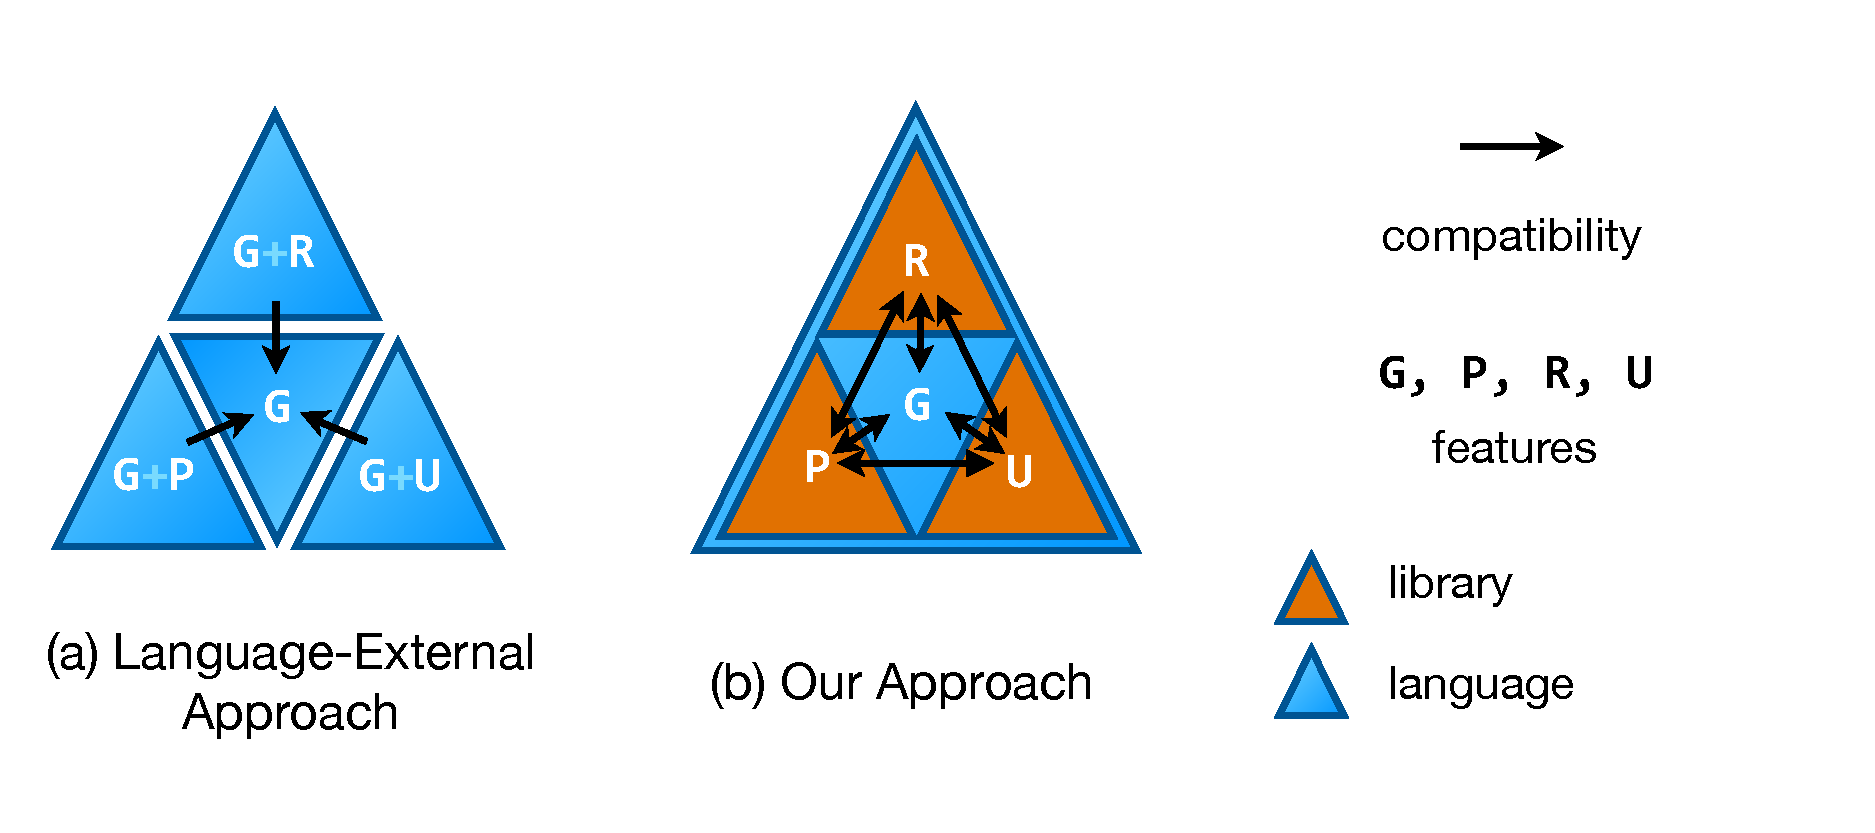
\includegraphics[scale=0.5]{approaches.pdf}
\end{center}
\vspace{-20px}
\caption{\small (a) With a language-oriented approach, novel constructs are packaged into separate languages. Users can only safely and naturally call into languages consisting of common constructs (often only the common target language, such as C or Java bytecode). (b) With a language-internal extensibility approach, there is one system providing a common internal language, where additional primitive constructs that strictly strengthen its static guarantees or perform specialized code generation are specified and distributed within libraries. \label{approaches}}
\end{figure*}

%As a result, domain-specific languages and new general-purpose abstractions alike have experienced relatively slow adoption in practice.
%
%Porting large codebases to new languages is difficult, and the dominant programming languages innovate slowly, so programming language.
%
%More specifically, such languages are neither \emph{internally extensible} because the language itself exposes only natural numbers and functions to its users, nor are they \emph{externally extensible} because no new behaviors can be added to the language's  implementation in a separate module from the one containing the initial implementation.

%This is the essence of a monolithic language implementation: it is impossible for anyone to modularly extend languages defined in this way. 


Internally-extensible programming languages promise to avoid these problems by providing researchers and domain experts with a language-supported mechanism for specifying new primitive types and operators.
Using such extensions, library developers need only consider which abstractions are most appropriate for their domain, without also considering whether these constructs can be exposed using abstractions appropriate to the domains of client code. Clients can simply import any necessary constructs when using a library that relies on them, preserving safety and ease-of-use without the use of  wrappers and glue code. We show this competing approach in Figure \ref{approaches}(b).

%Researchers and domain experts thus gain the ability to distribute new ideas for evaluation to a broader development community without requiring the approval of maintainers of mainstream languages, large-scale porting of code or explicit interoperability layers. 

Unfortunately, a significant challenge remains before such a mechanism is possible: balancing expressiveness with concerns about maintaining safety properties in the presence of arbitrary combinations of user-defined language extensions. {\color{red} transition here} Correctness properties of an extension itself should be modularly verifiable, so that its users can rely on it for verifying and compiling their own code. The mechanism must also ensure that desirable metatheoretic properties and global safety guarantees of the language cannot be weakened by extensions. And with multiple independently-developed extensions used at once, the mechanism must further guarantee that they cannot interfere with one another. 

In this paper, we will describe a language-internal extensibility mechanism called \emph{active typechecking and translation} (AT\&T) that allows developers to specify new typechecking rules and translation logic from within libraries. The AT\&T mechanism utilizes type-level computation of higher kind and integrates typed compilation techniques into the language to provide strong safety guarantees, while remaining straightforward and expressive.

AT\&T is general with respect to many choices about the type-level language, the typed internal language and syntax. Choices along these dimensions can affect both expressiveness and ease-of-use. We will begin in Sec. 2 by introducing a minimal system called $@\lambda$ (the ``actively-typed lambda calculus'') that distills the essence of the mechanism in a simply-typed, simply-kinded setting. This will allow us to fully and concisely formalize the language and compiler and give several key safety theorems. We will then continue in Sec. 3 by discussing variants of this mechanism based on other basic paradigms, considering dependently-typed functional languages and object-oriented languages, discussing trade-offs between expressivity and safety when doing so. We have developed a simple prototype called Ace and have used it to develop a number of full-scale language extensions as libraries. We will briefly discuss this language and these extensions in Sec. 4.

We note at the outset that AT\&T focuses on extending the static semantics of languages with fixed, though flexible, syntax. Language-internal syntax extension mechanisms have been developed in the past (e.g. SugarJ \cite{sugarj}) but they have also suffered from safety problems because grammar composition is not always safe when done in an  unconstrained manner. Constrained approaches that provide stronger safety guarantees have recently been outlined (e.g. Wyvern \cite{globaldsl13}) but we will leave integration of syntax extensions with semantic extensions as future work.

\section{From Externally-Extensible Implementations to Internally-Extensible Languages}
To understand the genesis of our internal extensibility mechanism, it is helpful to begin by considering why most implementations of programming languages are not even \emph{externally extensible}. Let us consider again Godel's T. 
In a functional implementation, its types and operators will invariably be represented using {closed} datatypes. For example, a simple implementation in Standard ML may be based around these datatypes:
\begin{lstlisting}
  datatype Type = Nat | Arrow of Type * Type
  datatype Exp = Var of var 
               | Lam of var * Type * Exp
               | Ap of Exp * Exp 
               | Z | S of Exp 
               | Natrec of Exp * Exp * Exp
\end{lstlisting}

The logic governing the typechecking phase as well as the initial compilation phase (we call this phase \emph{translation} to distinguish it from subsequent optimization phases) will proceed by exhaustive case analysis.
In an object-oriented implementation of Godel's T, we could instead represent types and operators as instances of subclasses of abstract classes \lstinline{Type} and \lstinline{Exp}. If typechecking and translation then proceed by the ubiquitous \emph{visitor pattern} \cite{visitor}, by dispatching against a {fixed} collection of known subclasses of \lstinline{Exp}, the same basic issue is encountered: there is no modular way to add new primitive types or operators to the implementation.
Indeed, this basic issue is the canonical example of the widely-discussed \emph{expression problem} \cite{wadler-expression}.

A number of language mechanisms have been proposed that allow new cases to be added to datatypes and functions  in a modular way. In functional languages, these are known as \emph{open datatypes} \cite{open-datatypes}. The language might allow you to add types and operators for products to an open variant of the above definitions  like this: 
\begin{lstlisting}
  newcase Prod of Type * Type extends Type
  newcase Pair of Exp * Exp extends Exp
  newcase PrL of Exp extends Exp
  newcase PrR of Exp extends Exp
\end{lstlisting}

The corresponding logic for functionality like typechecking and translation can then be specified for only the new cases, e.g.:
\begin{lstlisting}
  typeof PrL(e) = 
    case typeof e of 
      Prod(t1, _) => t1 
    | _ => raise TypeError("<message>")
\end{lstlisting}

If we allow users to define new modules containing definitions like these and link them into our compiler, we have succeeded in creating an externally-extensible language implementation, albeit one where safety is not guaranteed (we will return to this point shortly). We have not, however, created an extensible programming language, because other implementations of the language will not necessarily support the same mechanism. 
If our newly-introduced constructs are used at library interface boundaries, we introduce the same compatibility problems that developing a new standalone language can create. That is, \textbf{extending a language by extending a single implementation of it is equivalent to creating a new language}. Several prominent language ecosystems today are in a state where a prominent compiler has introduced extensions that many libraries have come to rely on, including the Glasgow Haskell Compiler and the GNU compilers for C and C++. We argue that this practice should be considered harmful.

A more appropriate and useful place for extensions like this is directly within libraries. To enable such use cases, the language must provide a mechanism that allows expert users to declare new type families, like \lstinline{Prod}, their associated operators, like \lstinline{Pair}, \lstinline{PrL} and \lstinline{PrR}, and their associated typechecking and translation logic. When a compiler encounters these declarations, it adds them to its internal representation of types and operators, as if they had been primitives of the language, so that when user-defined operators are used in expressions, the compiler can temporarily hand control over the typechecking and translation phases to them. Because the mechanism is {language-internal}, all compilers must support it to satisfy the language specification. Thus, library developers can use new primitive constructs at external interfaces more freely.

Statically-typed languages typically make a distinction between the expression language, where run-time logic is expressed, and the type-level language where, for example, datatypes and type aliases are statically declared. The description above suggests we may now need another layer in our language, an {extension language}, where users provide extension specifications. In fact, we will show that \textbf{the natural place for type system extensions is within the type-level language}. The intuition is that extensions will need to introduce and statically manipulate types and type families. Many languages already support notions of \emph{type-level computation} where types are manipulated as values at compile-time (see Sec. \ref{related} for examples of such languages). These are precisely the properties that such an extension language would have, so we unify the two.

\section{$\text{@}\lambda$}
\begin{figure}
\small
$$\begin{array}{rccl}	
\textbf{programs}                    &   \rho &  ::= & \pfam{\familyDf}{\progsort}\\
									&        &  \pipe & \pdef{t}{\kappa}{\tau}{\progsort}\\
									&        &  \pipe & e\\
									\\
\textbf{expressions} 				&	e	&	::=	&	\evar{x} \pipe 
														\elam{\evar{x}}{\tau}{e} \pipe 
														\eop{Fam}{op}{
															\taui
														}{
  												    		\splat{e}{1}{n}
														} \\
									& 		&		& 	\\
							
\hspace{-5pt}\textbf{type-level terms} 	& \tau 	& ::= 	& 	\tvar{t} \pipe 
														\tlam{t}{\kappa}{\tau} \pipe 
														\tapp{\tau_1}{\tau_2} \pipe \iintlit \pipe \iop{\tau_1}{\tau_2}
														\\
												
\text{type-level data}	 			& 		& \pipe	& 	 \tstr{str} \pipe \tunit \pipe 
														\tpair{\tau_{1}}{\tau_{2}} \pipe 
														\tfst{\tau} \pipe 
														\tsnd{\tau} 
														\\
									& & \pipe &          \tnil{\kappa} \pipe \tcons{\tau_1}{\tau_2} \pipe 
									                     \tfold{\tau_1}{\tau_2}{x}{y}{\tau_3}\\
\text{equivalence}  & & \pipe & 					\tifeq{\tau_{1}}{\tau_{2}}{\kappa}{\tau_{3}}{\tau_{4}} 
														\\														

\text{types} 						& 		& \pipe	& 	\ttypestd \\
										& & \pipe & \tfamcase{\tau}{Fam}{x}{\tau_1}{\tau_2}\\
																								
\text{denotations} 				& 		 & 	\pipe	&	\tden{\tau_2}{\tau_1} \pipe \terr\\
 & & \pipe & 
														\tdencase{\tau}{y}{x}{\tau_1}{\tau_2}
														 \\

\text{quoted IL}		&		&	\pipe	&	\titerm{\ghat} \pipe \titype{\dhat} \\

												\\
\textbf{kinds} 					& \kappa	&	::=	&	\kTypeBlur \pipe \dint \pipe
											    \kstr \pipe
												\kunit \pipe 
												\kpair{\kappa_{1}}{\kappa_{2}} \pipe 
												\klist{\kappa}
\\& & \pipe & \karrow{\kappa_1}{\kappa_2} \pipe 
												\kDen \pipe 
												\kIType \pipe \kITerm
												\\
												\\
\textbf{ops}		&	\theta	&	::= &	\topsempty \pipe 
												\topp{\theta}{\tops{op}{\kappai}{i}{a}{\tau}}\\
\textbf{ops signature}			& \Theta	&	::=	&	\kOpEmpty \pipe \kOp{\Theta}{op}{\kappai}\\
											 							&		&		&	\\
\textbf{internal terms} 				& 	\mathcal{G}[\textit{g},\textit{s}]	&	::=	&	\evar{x} \pipe 
												\ilam{\evar{x}}{\textit{s}}{\textit{g}} \pipe 
												\iapp{\textit{g}_{1}}{\textit{g}_{2}} \pipe
												\ifix{\evar{f}}{\textit{s}}{\textit{g}} \pipe
												\iintlit \\
							& 		& 	\pipe	& 
												\iop{\textit{g}_{1}}{\textit{g}_{2}} \pipe 
												\ipair{\textit{g}_{1}}{\textit{g}_{2}} \pipe 
												\ifst{\textit{g}} \pipe
												\isnd{\textit{g}} \\
									& & \pipe &  
												\iIfEq{\textit{g}_{1}}{\textit{g}_{2}}{\dint}{\textit{g}_{3}}{\textit{g}_{4}}\\
\text{abstracted} & \ghat & ::= &\mathcal{G}[\ghat, \dhat] \pipe \tvalof{\tau_2}{\tau_1} \pipe \iup{\tau} \\
\text{deabstracted}& \gamma & ::= & \mathcal{G}[\gamma, \sigma]\\
\\
\textbf{internal types}			&	\mathcal{S}[\textit{s}]	&	::=	&    \darrow{\textit{s}_1}{\textit{s}_2} \pipe
												\dint \pipe
												\dpair{\textit{s}_1}{\textit{s}_2}\\
\text{abstracted}					& \dhat & ::= & \mathcal{S}[\dhat] \pipe \trepof{\tau} \pipe \dup{\tau}\\
\text{dequoted}				& \dbar & ::= & \mathcal{S}[\dbar] \pipe \trepof{\tau}\\
\text{deabstracted}								& \sigma & ::= & \mathcal{S}[\sigma]\\
\end{array}$$
\caption{\small Syntax of \atlam. Variables $x$ are used in expressions and internal terms and $\tvar{t}$ in type-level terms. Names $\fvar{Fam}$ are family names (we assume that unique family names can be generated by some extrinsic mechanism) and $\opvar{op}$ for operator names. $\tstr{str}$ denotes string literals, $\iintlit$ denotes integer literals and $\oplus$ stands for binary operations over integers. The metavariables related to the internal language are written using generators $\mathcal{G}$ and $\mathcal{S}$ to avoid duplicating the syntax of common terms.\label{grammar}}
\end{figure}
Let us now make these ideas more concrete by developing a core calculus, and discuss how to address safety concerns that arise when giving users this level of control over the language. 

\subsection{Overview}
Our calculus, called @$\lambda$ for ``actively-typed lambda calculus'', is based on the simply-typed lambda calculus with simply-kinded type-level computation. That is, type-level terms themselves form a second-level simply-typed lambda calculus; we call the second level of types \emph{kinds} for clarity. Types themselves, which classify expressions, are type-level terms of kind $\star$ (following conventional notation \cite{fomega}), but there are also other kinds of type-level terms, including type-level lambda abstraction and other type-level data structures (we include type-level strings, nullary and binary products and primitive lists for the sake of our examples; see Sec. \ref{termination} for a discussion of what other kinds of data would be acceptable here). Type-level data and types can be compared for structural equality (i.e. a subset of kinds are comparable, discussed below).

Our calculus then introduces type-level mechanisms for introducing new type families and associated primitive operators. Operators specify their run-time semantics by giving a translation to a typed \emph{internal language}, here based on an expanded variant of Plotkin's PCF \cite{pfpl} for the sake of example (see Sec. \ref{target}). The abstract syntax for expressions, types, kinds and the typed internal language (consisting of \emph{internal types} and \emph{internal terms}) is shown in Figure \ref{grammar}. We will now discuss each of these components of the calculus with some examples.

We build in lambdas as the only binding structure in the language to simplify the core calculus. All other operators are associated with a type. For example, nat / tuples / records.

Operator families. 

Records: 
\subsection{Statics}
\begin{figure}
\small
\begin{mathpar}
\inferrule{
	\overbrace{\progOK{\emptyctx}{\fvarCtx_0}{\rho}}^{\text{\normalsize Kind Checking}}\\
	\overbrace{\pcompiles{\fvalCtx_0}{\rho}{\gamma}}^{\text{\normalsize Active Typechecking and Translation}}
}{
	\ptcc{\rho}{\gamma}
}
\end{mathpar}
\caption{\small Central Compilation Judgement of \atlam.}
\end{figure}
\begin{figure}
\small
$$\begin{array}{rcl}
\fvarCtx_0 & := & \fvarOfType{Arrow}{\kpair{\kTypeBlur}{\kTypeBlur}}{\kOpS{ap}{\kunit}}\\
 \fvalCtx_0 & := & \fval{Arrow}{\theta_0}{i}{\titype{\darrow{\trepof{\tfst{\tvar{i}}}}{\trepof{\tsnd{\tvar{i}}}}}}\\
 \theta_0 & := & \tops{ap}{\kunit}{i}{a}{x}%len(a)=2 and dencase a[0] of [[Arrow<(t1, t2)> => v1]] => dencase a[1] of [[t => v2]] => if t = t1 then [[t2 ==> up(v1) up(v2)]] else err else err else err else err}
\end{array}$$
\caption{\small The $\fvar{Arrow}$ type family is included by default as defined above. The definition of XXX,  written in terms of \textsf{fold}, has been alided for concision.}
\end{figure}
\begin{figure}
\small
$\fbox{\inferrule{}{\progOKX{\progsort}}}$
~~~$\tvarCtx ::= \emptyctx \pipe \tvarCtxX{t}{\kappa}$~~~
$\fCtx ::= \Sigma_0	 \pipe \fvarCtxX$
\begin{mathpar}
\inferrule[family decl kinding]{
	\fvar{Fam} \notin \fvarCtx\\
	\kEq{\kappaidx}\\
	\opType{\tvarCtx}{\fvarCtxX}{\theta}{\Theta}\\\\
	\tKind{\tvarCtx, \tvar{i}:{\kappaidx}}{\fvarCtxX}{\tau}{\kIType}\\
	\progOK{\tvarCtx}{\fvarCtxX}{\rho}
}{
	\progOKX{\pfam{\familyDf}{\rho}}
}

\inferrule[type-level bind kinding]{
	\tKindX{\tau}{\kappa}\\
	\progOK{\tvarCtxX{t}{\kappa}}{\fvarCtx}{\rho}
}{
	\progOKX{\pdef{t}{\kappa}{\tau}{\rho}}
}

\inferrule[exp kinding]{
	\exprOK{\tvarCtx}{\emptyctx}{\fvarCtx}{e}
}{
	\progOKX{e}
}
\end{mathpar}
$\fbox{$\tKindX{\theta}{\Theta}$}$
\begin{mathpar}
\inferrule[no ops]{ }{
	\tKindX{\topsempty}{\kOpEmpty}
}

\inferrule[ops]{
	\opType{\tvarCtx}{\fvarCtx}{\theta}{\Theta}\\
	\opvar{op} \notin \theta\\\\
	\tKind{\tvarCtx, \tOfKind{\tvar{i}}{\kappai}, \tOfKind{\tvar{a}}{\klist{\kDen}}}{\fvarCtx}{\tau}{\kDen}
}{
	\opType{\tvarCtx}{\fvarCtx}{\topp{\theta}{\tops{op}{\kappai}{i}{a}{\tau}}}{
	\kOp{\Theta}{op}{\kappai}}
}
\end{mathpar}
$\fbox{$\exprOKX{e}$}$
~~~$\itvarCtx ::= \emptyctx \pipe \itvarCtx, \evar{x}$
\begin{mathpar}
\inferrule[e-var-kind]{ }{
	\exprOK{\tvarCtx}{\itvarCtx, \evar{x}}{\fvarCtx}{\evar{x}}
}

\inferrule[e-lam-kind]{
	\tKindX{\tau}{\kTypeBlur}\\
	\exprOK{\tvarCtx}{\eivarCtxX{x}}{\fvarCtx}{e}
}{
	\exprOKX{\elam{\evar{x}}{\tau}{e}}
}

\inferrule[e-op-kind]{
	\fvarOfType{Fam}{\kappaidx}{\Theta} \in \fvarCtx\\
	\kOpS{op}{\kappai} \in \Theta\\
	\tKindX{\taui}{\kappai}\\\\
	\exprOKX{e_1}\\
	\cdots\\
	\exprOKX{e_n}
}{
	\exprOKX{\eop{Fam}{op}{\taui}{\splat{e}{1}{n}}}
}
\end{mathpar}
\caption{\small Kinding for programs. Variable contexts $\tvarCtx$ and $\itvarCtx$ obey standard structural properties. Kinding for type-level terms in Figure \ref{kindtl}. \ \label{kindprof}}
\end{figure}
\begin{figure}
\small
$\fbox{\inferrule{}{\pcompilesX{\rho}}}$
~~~$\fvalCtx ::= \fvalCtx_0 \pipe \fvalCtxX{\fvalDf}$
\begin{mathpar}
\inferrule[att-fam]{
	\pcompiles{\fvalCtxX{\fvalDf}}{\rho}{\gamma}
}{
	\pcompilesX{\pfam{\familyDf}{\rho}}
}

\inferrule[att-def]{
	\tEvalX{\tau}{\tau'}\\
	\pcompilesX{\subst{\tau'}{\tvar{t}}{\rho}}
}{
	\pcompilesX{\pdef{t}{\kappa}{\tau}{\rho}}
}

\inferrule[att-exp]{
	\ecompiles{\emptyctx}{\fvalCtx}{e}{\tau}{\ghat}\\
	\eraseX{\ghat}{\gamma}
}{
	\pcompilesX{e}
}
\end{mathpar}
$\fbox{\inferrule{}{\ecompilesX{e}{\tau}{\ghat}}}$
~~~$\etCtx ::= \emptyctx \pipe \etCtxX{x}{\tau}$
\begin{mathpar}
\inferrule[att-var]{ }{
	\ecompiles{\etCtxX{x}{\tau}}{\fvalCtx}{\evar{x}}{\tau}{\evar{x}}
}

\inferrule[att-lam]{
	\tEvalX{\tau_1}{\ttype{Fam}{\tauidx}}\\
	\ecompiles{\etCtxX{x}{\ttype{Fam}{\tauidx}}}{\fvalCtx}{e}{\tau_2}{\ghat}\\\\
	\tauisdel{Arrow}{\fvalCtx}{Fam}{\tauidx}{\dbar}\\
}{
	\ecompiles{\etCtx}{\fvalCtx}{\elam{\evar{x}}{\tau_1}{e}}{\ttype{Arrow}{\tpair{\ttype{Fam}{\tauidx}}{\tau_2}}}{\ilam{\evar{x}}{\dbar}{\ghat}}
}

\inferrule[att-op]{
	\fvalDf \in \fvalCtx\\
	\tops{op}{\kappai}{i}{a}{\tauop} \in \theta\\
	\tEvalX{\taui}{\taui'}\\\\
	\ecompiles{\etCtx}{\fvalCtx}{e_1}{\tau_1}{\ghat_1}~~~~
	\cdots~~~~
	\ecompiles{\etCtx}{\fvalCtx}{e_n}{\tau_n}{\ghat_n}\\
	\left\{\text{$\begin{array}{c}
		\left[\text{$\begin{array}{r}
			\taui'/\tvar{i}\\
			\tden{\titerm{\ghat_1}}{\tau_1} :: \cdots :: \tden{\titerm{\ghat_n}}{\tau_n} :: \tnil{\kDen}/\tvar{a}
			\end{array}$}\right]\tauop\\
		\Downarrow\\
		\tden{\titerm{\ghat}}{\ttype{Fam'}{\tauidx}}
		\end{array}$}\right\}\\
	\tauisdel{Fam}{\fvalCtx}{Fam'}{\tauidx}{\dbar}\\
	\eCtxTogCtx{Fam}{\fvalCtx}{\etCtx}{\gtCtx}\\
	\checkRC{\gtCtx}{Fam}{\fvalCtx}{\ghat}{\dbar}
}{
	\ecompiles{\etCtx}{\fvalCtx}{\eop{Fam}{op}{\taui}{\splat{e}{1}{n}}}{\ttype{Fam'}{\tauidx}}{\ghat}
}
\end{mathpar}
\caption{\small Active typechecking and translation}
\end{figure}
\begin{figure}
\small

$\fbox{\inferrule{}{\tKindX{\tau}{\kappa}}}$
\begin{mathpar}
\small
\inferrule[var kind]{
}{
  \tKind{\tvarCtxX{t}{\kappa}}{\fvarCtx}{\tvar{t}}{\kappa}
}

\inferrule[k-arrow intro]{
  \tKind{\tvarCtxX{t}{\kappa_1}}{\fvarCtx}{\tau}{\kappa_2}
}{
  \tKindX{\tlam{t}{\kappa_1}{\tau}}{\karrow{\kappa_1}{\kappa_2}}
}

\inferrule[k-arrow elim]{
  \tKindX{\tau_1}{\karrow{\kappa_1}{\kappa_2}}\\
  \tKindX{\tau_2}{\kappa_1}
}{
  \tKindX{\tapp{\tau_1}{\tau_2}}{\kappa_2}
}
\\
\text{\color{gray} (standard statics for integers, strings, products and lists omitted)}
\\
%%
%%\inferrule{ }{
%%	\tKindX{\tstr{str}}{\kstr}
%%}(\text{str}^I_\tau)
%%
%%\inferrule{ }{
%%	\tKindX{\tunit}{\kunit}
%%}(\text{1}^I_\tau)
%%
%%\inferrule{
%%	\tKindX{\tau_1}{\kappa_1}\\
%%	\tKindX{\tau_2}{\kappa_2}
%%}{
%%	\tKindX{\tpair{\tau_1}{\tau_2}}{\kpair{\kappa_1}{\kappa_2}}
%%}({\times}^I_\tau)
%%
%%\inferrule{
%%	\tKindX{\tau}{\kpair}{\kappa_1}{\kappa_2}
%%}{
%%	\tKindX{\tfst{\tau}}{\kappa_1}
%%}({\times}^{E1}_\tau)
%%
%%\inferrule{
%%	\tKindX{\tau}{\kpair}{\kappa_1}{\kappa_2}
%%}{
%%	\tKindX{\tsnd{\tau}}{\kappa_2}
%%}({\times}^{E2}_\tau)
%%\inferrule{ }{
%%\inferrule{
%%	\tKindX{\tau_{1}}{\kappa_{1}}\\
%%	\tKindX{\tau_{2}}{\kappa_{2}}
%%}{
%%	\tKindX{\tpair{\tau_{1}}{\tau_{2}}}{\kpair{\kappa_{1}}{\kappa_{2}}}
%%}~(\times_\tau)
%%
%%\inferrule{
%%	\tKindX{\tau}{\kpair{\kappa_{1}}{\kappa_{2}}}
%%}{
%%	\tKindX{\tfst{\tau}}{\kappa_{1}}
%%}~(\text{fst}_\tau)
%%
%%\inferrule{
%%	\tKindX{\tau}{\kpair{\kappa_{1}}{\kappa_{2}}}
%%}{
%%	\tKindX{\tsnd{\tau}}{\kappa_{2}}
%%}~(\text{snd}_\tau)
%%
%% TODO: list
\inferrule[eq kind]{
	\kEq{\kappa}\\
	\tKindX{\tau_1}{\kappa}\\
	\tKindX{\tau_2}{\kappa}\\\\
	\tKindX{\tau_3}{\kappa'}\\
	\tKindX{\tau_4}{\kappa'}
}{
	\tKindX{\tifeq{\tau_1}{\tau_2}{\kappa}{\tau_3}{\tau_4}}{\kappa'}
}

\inferrule[type intro]{
	\fvarOfTypeDf \in \fvarCtx\\\\
	\tKind{\tvarCtx}{\fvarCtx}{\tauidx}{\kappaidx}
}{
	\tKindX{\ttype{Fam}{\tauidx}}{\kTypeBlur}
}

\inferrule[type elim]{
	\fvarOfTypeDf \in \fvarCtx\\
	\tKindX{\tau}{\kTypeBlur}\\
	\tKind{\tvarCtxX{x}{\kappaidx}}{\fvarCtx}{\tau_0}{\kappa}\\
	\tKindX{\tau_1}{\kappa}
}{
	\tKind{\tvarCtx}{\fvarCtx}{\tfamcase{\tau}{Fam}{x}{\tau_0}{\tau_1}}{\kappa}
}

\inferrule[den intro valid]{
	\tKindX{\tautype}{\kTypeBlur}\\
	\tKindX{\tauval}{\kITerm}
}{
	\tKindX{\tden{\tauval}{\tautype}}{\kDen}
}

\inferrule[den intro err]{ }{
	\tKindX{\terr}{\kDen}
}

\inferrule[den elim]{
	\tKindX{\tauden}{\kDen}\\
	\tKind{\tvarCtx, \tOfKind{\tvar{x}}{\kITerm}, \tOfKind{\tvar{y}}{\kTypeBlur}}{\fvarCtx}{\tau_1}{\kappa}\\
	\tKindX{\tau_2}{\kappa}
}{
	\tKindX{\tdencase{\tauden}{y}{x}{\tau_1}{\tau_2}}{\kappa}
}

\inferrule[iterm intro]{
	\isIterm{\tvarCtx}{\emptyctx}{\fvarCtx}{\ghat}
}{
	\tKindX{\titerm{\ghat}}{\kITerm}
}

\inferrule[itype intro]{
	\isItype{\tvarCtx}{\fvarCtx}{\dhat}
}{
	\tKindX{\titype{\dhat}}{\kIType}
}
\end{mathpar}
$\fbox{$\kEq{\kappa}$}$
\begin{mathpar}
\inferrule[t-eq]{ }{
	\kEq{\kTypeBlur}
}

\inferrule[z-eq]{ }{
	\kEq{\dint}
}

\inferrule[str-eq]{ }{
	\kEq{\kstr}
}

\inferrule[u-eq]{ }{
	\kEq{\kunit}
}

\inferrule[prod-eq]{
	\kEq{\kappa_1}\\\\
	\kEq{\kappa_2}
}{
	\kEq{\kpair{\kappa_1}{\kappa_2}}
}

\inferrule[list-eq]{
	\kEq{\kappa}
}{
	\kEq{\klist{\kappa}}
}
\end{mathpar}
$\fbox{$\isItermX{\ghat}$}$
\begin{mathpar}
\inferrule[i-var kind]{ }{
	\isIterm{\tvarCtx}{\eivarCtxX{x}}{\fvarCtx}{\evar{x}}
}

\inferrule[i-lam kind]{
	\isItypeX{\dhat}\\
	\isIterm{\tvarCtx}{\eivarCtxX{x}}{\fvarCtx}{\ghat}
}{
	\isItermX{\ilam{\evar{x}}{\dhat}{\ghat}}
}

\inferrule[i-fix kind]{
	\isItypeX{\dhat}\\
	\isIterm{\tvarCtx}{\eivarCtxX{x}}{\fvarCtx}{\ghat}
}{
	\isItermX{\ifix{\evar{f}}{\dhat}{\ghat}}
}
\\
\text{\color{gray} (omitted forms have trivially recursive rules)}\\\vspace{-3pt}
\\
\inferrule[iterm unquote kind]{
	\tKindX{\tau}{\kITerm}
}{
	\isItermX{\iup{\tau}}
}

\inferrule[val from den kind]{
	\tKindX{\tautype}{\kTypeBlur}\\
	\tKindX{\tauval}{\kITerm}
}{
	\isItermX{\tvalof{\tauval}{\tautype}}
}
\end{mathpar}
$\fbox{$\isItypeX{\dhat}$}$
\begin{mathpar}
\inferrule[i-int kind]{ }{
	\isItypeX{\dint}
}

\inferrule[i-prod kind]{
	\isItypeX{\dhat_1}\\
	\isItypeX{\dhat_2}
}{
	\isItypeX{\dpair{\dhat_1}{\dhat_2}}
}

\inferrule[i-arrow kind]{
	\isItypeX{\dhat_1}\\
	\isItypeX{\dhat_2}
}{
	\isItypeX{\darrow{\dhat_1}{\dhat_2}}
}
\\
\inferrule[itype unquote kind]{
	\tKindX{\tau}{\kIType}
}{
	\isItypeX{\dup{\tau}}
}

\inferrule[rep from type kind]{
	\tKindX{\tau}{\kTypeBlur}
}{
	\isItypeX{\trepof{\tau}}
}
\end{mathpar}
\caption{\small Kinding for type-level terms}
\end{figure}

\begin{figure}
\small
$\fbox{$\tEvalX{\tau}{\tau'}$}$
\begin{mathpar}
\inferrule[tl-lam eval]{ }{
	\tEvalX{\tlam{t}{\kappa}{\tau}}{\tlam{t}{\kappa}{\tau}}
}

\inferrule[tl-ap eval]{
	\tEvalX{\tau_1}{\tlam{t}{\kappa}{\tau}}\\
	\tEvalX{\tau_2}{\tau_2'}\\
	\tEvalX{\subst{\tau_2'}{\tvar{t}}{\tau}}{\tau'}
}{
	\tEvalX{\tapp{\tau_1}{\tau_2}}{\tau'}
}

\text{\color{gray} (standard evaluation rules for integers, strings, products and lists omitted)}

\inferrule[tl-eq eval eq]{
	\tEvalX{\tau_1}{\tau_1'}\\
	\tEvalX{\tau_2}{\tau_1'}\\
	\tEvalX{\tau_3}{\tau_3'}
}{
	\tEvalX{\tifeq{\tau_1}{\tau_2}{\kappa}{\tau_3}{\tau_4}}{\tau_3'}
}

\inferrule[tl-eq eval neq]{
	\tEvalX{\tau_1}{\tau_1'}\\
	\tEvalX{\tau_2}{\tau_2'}\\
	\tau_1' \neq \tau_2'\\
	\tEvalX{\tau_4}{\tau_4'}
}{
	\tEvalX{\tifeq{\tau_1}{\tau_2}{\kappa}{\tau_3}{\tau_4}}{\tau_4'}
}

\inferrule[type eval]{
	\tEvalX{\tauidx}{\tauidx'}
}{
	\tEvalX{\ttype{Fam}{\tauidx}}{\ttype{Fam}{\tauidx'}}
}

\inferrule[famcase eval match]{
	\tEvalX{\tau}{\ttype{Fam}{\tauidx}}\\
	\tEvalX{\subst{\tauidx}{\tvar{x}}{\tau_1}}{\tau_1'}
}{
	\tEvalX{\tfamcase{\tau}{Fam}{x}{\tau_1}{\tau_2}}{\tau_1'}
}

\inferrule[famcase eval fail]{
	\tEvalX{\tau}{\ttype{Fam'}{\tauidx}}\\
	\fvar{Fam} \neq \fvar{Fam'}\\
	\tEvalX{\tau_2}{\tau_2'}
}{
	\tEvalX{\tfamcase{\tau}{Fam}{x}{\tau_1}{\tau_2}}{\tau_2'}
}

\inferrule[den eval]{
	\tEvalX{\tautype}{\tautype'}\\
	\tEvalX{\tauval}{\tauval'}
}{
	\tEvalX{\tden{\tauval}{\tautype}}{\tden{\tauval'}{\tautype'}}
}

\inferrule[err eval]{ }{
	\tEvalX{\terr}{\terr}
}

\inferrule[dencase eval valid]{
	\tEvalX{\tauden}{\tden{\tauval}{\tautype}}\\
	\tEvalX{[\tautype/\tvar{x}, \titerm{\tvalof{\tauval}{\tautype}}/\tvar{y}]\tau_1}{\tau_1'}
}{
	\tEvalX{\tdencase{\tauden}{y}{x}{\tau_1}{\tau_2}}{\tau_1'}
}

\inferrule[dencase eval err]{
	\tEvalX{\tauden}{\terr}\\
	\tEvalX{\tau_2}{\tau_2'}
}{
	\tEvalX{\tdencase{\tauden}{y}{x}{\tau_1}{\tau_2}}{\tau_2'}
}
\\
\inferrule[iterm quote eval]{
	\tiEvalX{\ghat}{\ghat'}
}{
	\tEvalX{\titerm{\ghat}}{\titerm{\ghat'}}
}

\inferrule[itype quote eval]{
	\tiEvalX{\dhat}{\dhat'}
}{
	\tEvalX{\titype{\dhat}}{\titype{\dhat'}}
}
\end{mathpar}
$\fbox{$\tiEvalX{\ghat}{\ghat'}$}$
\begin{mathpar}
\inferrule[i-var eval]{ }{
	\tiEvalX{\evar{x}}{\evar{x}}
}

\inferrule[i-lam eval]{
	\tiEvalX{\dhat}{\dhat'}\\
	\tiEvalX{\ghat}{\ghat'}
}{
	\tiEvalX{\ilam{\evar{x}}{\dhat}{\ghat}}{\ilam{\evar{x}}{\dhat'}{\ghat'}}
}

\inferrule[i-fix eval]{
	\tiEvalX{\dhat}{\dhat'}\\
	\tiEvalX{\ghat}{\ghat'}
}{
	\tiEvalX{\ifix{\evar{f}}{\dhat}{\ghat}}{\ifix{\evar{f}}{\dhat'}{\ghat'}}
}
\\
\text{\color{gray} (omitted forms have trivially recursive rules)}
\\
\inferrule[iterm unquote eval]{
	\tEvalX{\tau}{\tau'}
}{
	\tiEvalX{\iup{\tau}}{\iup{\tau'}}
}

\inferrule[val from den eval]{
	\tEvalX{\tautype}{\tautype'}\\
	\tEvalX{\tauval}{\tauval'}
}{
	\tiEvalX{\tvalof{\tauval}{\tautype}}{\tvalof{\tauval'}{\tautype'}}
}
\end{mathpar}
$\fbox{$\tiEvalX{\sigma}{\sigma'}$}$
\begin{mathpar}
\inferrule[i-int eval]{ }{
	\tiEvalX{\dint}{\dint}
}

\inferrule[i-prod eval]{
	\tiEvalX{\dhat_1}{\dhat_1'}\\
	\tiEvalX{\dhat_2}{\dhat_2'}
}{
	\tiEvalX{\dpair{\dhat_1}{\dhat_2}}{\dpair{\dhat_1'}{\dhat_2'}}
}

\inferrule[i-arrow eval]{
	\tiEvalX{\dhat_1}{\dhat_1'}\\
	\tiEvalX{\dhat_2}{\dhat_2'}
}{
	\tiEvalX{\darrow{\dhat_1}{\dhat_2}}{\darrow{\dhat_1'}{\dhat_2'}}
}

\inferrule[itype unquote eval]{
	\tEvalX{\tau}{\tau'}
}{
	\tiEvalX{\dup{\tau}}{\dup{\tau'}}
}

\inferrule[rep from type eval]{
	\tEvalX{\tau}{\tau'}
}{
	\tiEvalX{\trepof{\tau}}{\trepof{\tau'}}
}
\end{mathpar}
\caption{\small Evaluation semantics for type-level terms}
\end{figure}

\begin{figure}
\small
$\fbox{\inferrule{}{\delfromtau{Fam}{\fvalCtx}{\tau}{\dbar}}}$
~~~$\fvalCtx ::= \fvalCtx_0 \pipe \fvalCtx, \fvalDf$
\begin{mathpar}
\inferrule[abs rep from type]{
	\fval{Fam'}{\theta}{i}{\tau} \in \fvalCtx\\
	\tEvalX{[\tauidx/\tvar{i}]\tau}{\titype{\dhat}}\\
	\ddbarX{\dhat}{\dbar}
}{
	\tauisdel{Fam}{\fvalCtx}{Fam'}{\tauidx}{\dbar}
}
\end{mathpar}
$\fbox{\inferrule{}{\ddbarX{\dhat}{\dbar}}}$
\begin{mathpar}
\inferrule[abs int]{ }{
	\ddbarX{\dint}{\dint}
}

\inferrule[abs arrow]{
	\ddbarX{\dhat_1}{\dbar_1}\\
	\ddbarX{\dhat_2}{\dbar_2}
}{
	\ddbarX{\darrow{\dhat_1}{\dhat_2}}{\darrow{\dbar_1}{\dbar_2}}
}

\inferrule[abs prod]{
	\ddbarX{\dhat_1}{\dbar_1}\\
	\ddbarX{\dhat_2}{\dbar_2}
}{
	\ddbarX{\dpair{\dhat_1}{\dhat_2}}{\dpair{\dbar_1}{\dbar_2}}
}

\inferrule[abs+cancel unquote]{
	\ddbarX{\dhat}{\dbar}
}{
	\ddbarX{\dup{\titype{\dhat}}}{\dbar}
}

\inferrule[abs rep from type visible]{
	\fvalDf \in \fvalCtx\\
	\tEvalX{[\tauidx/\tvar{i}]\tau}{\titype{\dhat}}\\
	\ddbarX{\dhat}{\dbar}
}{
	\ddbarX{\trepof{\ttype{Fam}{\tauidx}}}{\dbar}
}

\inferrule[abs rep from type hidden]{
	\fvar{Fam} \neq \fvar{Fam'}
}{
	\ddbarX{\trepof{\ttype{Fam'}{\tauidx}}}{\trepof{\ttype{Fam'}{\tauidx}}}
}
\end{mathpar}
$\fbox{\inferrule{}{\eCtxTogCtxX{\etCtx}{\gtCtx}}}$
~~~$\gtCtx ::= \emptyctx \pipe \gtCtxX{x}{\dbar}$
\begin{mathpar}
\inferrule[abs empty]{ }{
	\eCtxTogCtxX{\emptyctx}{\emptyctx}
}

\inferrule[abs ctx]{
	\eCtxTogCtxX{\etCtx}{\gtCtx}\\
	\delfromtau{Fam}{\fvalCtx}{\tau}{\dbar}
}{
	\eCtxTogCtxX{\etCtxX{x}{\tau}}{\gtCtxX{x}{\dbar}}
}
\end{mathpar}
$\fbox{\inferrule{}{\checkRCX{\ghat}{\dbar}}}$
\begin{mathpar}
\inferrule[abs i-var]{ }{
	\checkRC{\gtCtxX{x}{\dbar}}{Fam}{\fvalCtx}{\evar{x}}{\dbar}
}

\inferrule[abs i-lam]{
	\ddbarX{\dhat_1}{\dbar_1}\\
	\checkRC{\gtCtxX{x}{\dbar_1}}{Fam}{\fvalCtx}{\gamma}{\dbar_2}
}{
	\checkRCX{\ilam{x}{\dhat_1}{\gamma}}{\darrow{\dbar_1}{\dbar_2}}
}

\inferrule[abs i-ap]{
	\checkRCX{\ghat_1}{\darrow{\dbar_1}{\dbar_2}}\\\\
	\checkRCX{\ghat_2}{\dbar_1}
}{
	\checkRCX{\iapp{\ghat_1}{\ghat_2}}{\dbar_2}
}

\inferrule[abs i-fix]{
	\ddbarX{\dhat}{\dbar}\\
	\checkRC{\gtCtxX{x}{\dbar}}{Fam}{\fvalCtx}{\ghat}{\dbar}
}{
	\checkRCX{\ifix{x}{\dhat}{\ghat}}{\dbar}
}
\\
\text{\color{gray} (standard statics for integers and products omitted)}
\\
%\inferrule[abs int]{ }{
%	\checkRCX{\iintlit}{\dint}
%}
%
%\inferrule[abs op]{
%	\checkRCX{\gamma_1}{\dint}\\
%	\checkRCX{\gamma_2}{\dint}
%}{
%	\checkRCX{\iop{\gamma_1}{\gamma_2}}{\dint}
%}
%
%\inferrule[abs pair]{
%	\checkRCX{\gamma_1}{\dbar_1}\\
%	\checkRCX{\gamma_2}{\dbar_2}
%}{
%	\checkRCX{\ipair{\gamma_1}{\gamma_2}}{\dpair{\dbar_1}{\dbar_2}}
%}
%
%\inferrule[abs fst]{
%	\checkRCX{\gamma}{\dpair{\dbar_1}{\dbar_2}}
%}{
%	\checkRCX{\ifst{\gamma}}{\dbar_1}
%}
%
%\inferrule[abs snd]{
%	\checkRCX{\gamma}{\dpair{\dbar_1}{\dbar_2}}
%}{
%	\checkRCX{\isnd{\gamma}}{\dbar_2}
%}
%
\inferrule[abs if eq]{
	\checkRCX{\ghat_1}{\dint}\\
	\checkRCX{\ghat_2}{\dint}\\\\
	\checkRCX{\ghat_3}{\dbar}\\
	\checkRCX{\ghat_4}{\dbar}
}{
	\checkRCX{\iIfEq{\ghat_1}{\ghat_2}{\dint}{\ghat_3}{\ghat_4}}{\dbar}
}

\inferrule[abs iterm unquote]{
	\checkRCX{\ghat}{\dbar}
}{
	\checkRCX{\iup{\titerm{\ghat}}}{\dbar}
}

\inferrule[abs val from den visible]{
	\tauisdel{Fam}{\fvalCtx}{Fam}{\tauidx}{\dbar}\\
	\checkRCX{\ghat}{\dbar}
}{
	\checkRCX{\tvalof{\titerm{\ghat}}{\ttype{Fam}{\tauidx}}}{\dbar}
}

\inferrule[abs val from den hidden]{
	\fvar{Fam} \neq \fvar{Fam'}\\
	\tauisdel{Fam}{\fvalCtx}{Fam'}{\tauidx}{\dbar}\\
	\checkRCX{\ghat}{\dbar}
}{
	\checkRCX{\tvalof{\titerm{\ghat}}{\ttype{Fam'}{\tauidx}}}{\trepof{\ttype{Fam'}{\tauidx}}}
}
\end{mathpar}
\caption{\small Abstracted internal typing}
\end{figure}
\begin{figure}
\small
$\fbox{\inferrule{}{\eraseX{\dbar}{\sigma}}}$
\begin{mathpar}
\inferrule[deabs int]{ }{
	\eraseX{\dint}{\dint}
}

\inferrule[deabs arrow]{
	\eraseX{\dbar_1}{\sigma_1}\\\\
	\eraseX{\dbar_2}{\sigma_2}
}{
	\eraseX{\darrow{\dbar_1}{\dbar_2}}{\darrow{\sigma_1}{\sigma_2}}
}

\inferrule[deabs prod]{
	\eraseX{\dbar_1}{\sigma_1}\\\\
	\eraseX{\dbar_2}{\sigma_2}
}{
	\eraseX{\dpair{\dbar_1}{\dbar_2}}{\dpair{\sigma_1}{\sigma_2}}
}

\inferrule[deabs  rep from type hidden]{
	\fvalDf \in \fvalCtx\\
	\tEvalX{[\tauidx/\tvar{i}]\tau}{\titype{\dhat}}\\\\
	\ddbarX{\dhat}{\dbar}\\
	\eraseX{\dbar}{\sigma}
}{
	\eraseX{\trepof{\ttype{Fam}{\tauidx}}}{\sigma}
}
\end{mathpar}
$\fbox{\inferrule{}{\eraseX{\ghat}{\gamma}}}$
\begin{mathpar}
\inferrule[deabs i-var]{ }{
	\eraseX{\evar{x}}{\evar{x}}
}

\inferrule[deabs i-lam]{
	\ddbar{\_}{\fvalCtx}{\dhat}{\dbar}\\
	\eraseX{\dbar}{\sigma}\\
	\eraseX{\ghat}{\gamma}
}{
	\eraseX{\ilam{x}{\dhat}{\ghat}}{\ilam{x}{\sigma}{\gamma}}
}

%\inferrule[deabs ap]{
%	\eraseX{\ghat_1}{\ghat_1}\\
%	\eraseX{\ghat_2}{\ghat_2}
%}{
%	\eraseX{\iapp{\ghat_1}{\ghat_2}}{\iapp{\ghat_1}{\ghat_2}}
%}
%
\inferrule[deabs i-fix]{
	\ddbar{\_}{\fvalCtx}{\dhat}{\dbar}\\
	\eraseX{\dbar}{\sigma}\\
	\eraseX{\ghat}{\gamma}
}{
	\eraseX{\ifix{x}{\dhat}{\ghat}}{\ifix{x}{\sigma}{\gamma}}
}
\\
\text{\color{gray} (omitted forms have trivially recursive rules)}
\\
\inferrule[deabs unquote]{
	\eraseX{\ghat}{\gamma}
}{
	\eraseX{\iup{\titerm{\ghat}}}{\gamma}
}

\inferrule[deabs val from den hidden]{
	\eraseX{\ghat}{\gamma}
}{
	\eraseX{\tvalof{\titerm{\ghat}}{\ttype{Fam}{\tauidx}}}{\gamma}
}
\end{mathpar}
\caption{\small Deabstraction rules}
\end{figure}
%
%family RECORD of (string, type) dict {
%  new(idx, args. foldl (fn (x, y) => 
%  get[field : string](idx. case find(idx, field) of SOME t => t | _ => err)

\section{Safety of @$\lambda$}

\subsection{Dependent Kinds}
\section{Active Typechecking and Translation in Ace}
\section{Related Work}
\subsection{Type-Level Computation} %Haskell, Ur and $\Omega$mega
System XX with simple case analysis provides the basis of type-level computation in Haskell (where type-level functions are called type families \cite{Chakravarty:2005:ATC}). Ur uses type-level records and names to support typesafe metaprogramming, with applications to web programming \cite{conf/pldi/Chlipala10}. $\Omega$mega adds algebraic data types at the type-level, using these to increase the expressive power of algebraic data types at the expression level \cite{conf/cefp/SheardL07}. Dependently-typed languages blur the traditional phase separation between types and expressions, so type-level computation is often implicitly used (though not always in its most general form, e.g. Deputy \cite{conf/icfp/ChenX05}, ATS \cite{conf/esop/ConditHAGN07}.)

\subsection{Run-Time Indirection}
{\it Operator overloading} \cite{vanWijngaarden:Mailloux:Peck:Koster:Sintzoff:Lindsey:Meertens:Fisker:acta:1975} and {\it metaobject dispatch} \cite{Kiczales91} are run-time protocols that translate operator invocations into function calls. The function is typically selected according to the type or value of one or more operands. These protocols share the notion of {\it inversion of control} with type-level specification. However, type-level specification is a {\it compile-time} protocol focused on enabling specialized verification and implementation strategies, rather than simply enabling run-time indirection.

\subsection{Term Rewriting Systems}
Many languages and tools allow developers to rewrite expressions according to custom rules. These can broadly be classified as {\it term rewriting systems}. Macro systems, such as those characteristic of the LISP family of languages \cite{mccarthy1978history}, are the most prominent example. Some compile-time metaprogramming systems also allow users to manipulate syntax trees (e.g. MetaML \cite{Sheard:1999:UMS}), and external rewrite systems also exist for many languages.
These facilities differ from type-level specification in one or more of the following ways:

\begin{enumerate}
\item In type-level specification, the type of a value is determined separately from its representation; in fact, the same representation may be generated by multiple types. 
\item We draw a distinction between the metalanguage, used to specify types and compile-time logic, the source grammar, used to describe run-time behavior, and the internal language, used to implement this behavior. Term rewriting systems generally do not draw this distinction. By doing so, each component language can be structured and constrained as appropriate for its distinct role, as we show.
%\item With type-level specification, dispatch to a type-level function occurs implicitly on the basis of the structure of an expression. In contrast, most term-rewriting systems operate by  explicit invocation of a macro or specialized syntax. Some LISP macro systems have explored pattern-based dispatch (e.g. A*\cite{fowler2010domain}, EPP\cite{fowler2010domain}) and macro systems for object-oriented languages, like OpenC++ \cite{fowler2010domain} and OpenJava \cite{fowler2010domain}, do offer a somewhat limited form of operation-based dispatch.
\item Many common macro systems and metaprogramming facilities operate at run-time. Compilers for some forms of LISP employ aggressive compile-time specialization techniques to attempt to minimize this overhead. Static and staged term-rewriting systems also exist (e.g. OpenJava\cite{TatM:OpenJCBMSJ}, Template Haskell\cite{SheardPeytonJones:Haskell-02}, MetaML \cite{Sheard:1999:UMS} and others). 
\end{enumerate}

\subsection{Language Frameworks}
When the mechanisms available in an existing language prove insufficient, researchers and domain experts must design a new language. A number of tools have been developed to assist with this task, including compiler generators, language workbenches and domain-specific language frameworks (cf \cite{fowler2010domain}).

A major barrier to adoption is the fact that interoperability is intrinsically problematic. Even languages which target a common platform, such as the Java Virtual Machine, can only interact using its limited set of primitives. Specialized typing rules are not checked at language boundaries, performance often suffers, and the syntax can be unnatural, particularly for languages which differ significantly from the platform's native language (e.g. Java).

Instead of focusing on defining standalone languages, type-level specification gives greater responsibility in a granular manner to libraries. In this way, a range of constructs can coexist within the same program and, assuming that it can be shown by some method that various constructs are safely composable, be mixed and matched. The main limitation is that the protocol requires defining a fixed source grammar, whereas a specialized language has considerable flexibility in that regard. Nevertheless, as Ace shows, a simple grammar can be used quite flexibly.
\subsection{Extensible Compilers}
An alternative methodology is to implement language features granularly as compiler extensions. As discussed in Section 1, existing designs suffer from the same problems related to composability, modularity\-, safety and security as extensible languages, while also adding the issue of language fragmentation.

Type-level specification can in fact be implemented within a compiler, rather than provided as a core language feature. This would resolve some of the issues, as described in this paper. However, by leveraging type-level computation to integrate the protocol directly into the language, we benefit from common module systems and other shared infrastructure. We also avoid the fragmentation issue.
\subsection{Specification Languages}
Several {\it specification languages} (or {\it logical frameworks}) based on these theoretical formulations exist, including the OBJ family of languages (e.g. CafeOBJ \cite{Diaconescu-Futatsugi01}). They provide support for verifying a program against a language specification, and can automatically execute these programs as well in some cases. The  language itself specifies which verification and execution strategies are used.

Type-determined compilation takes a more concrete approach to the problem, focusing on combining {\it implementations} of different\- logics, rather than simply their specifications. In other words, it focuses on combining {\it type checkers} and {\it implementation strategies} rather than more abstract representations of a language's type system and dynamic semantics. In Section 4, we outlined a preliminary approach based on proof assistant available for the type-level language to unify these approaches, and we hope to continue this line of research in future work.

CANT GUARANTEE THAT SPECIFICATIONS ARE ACTUALLY DECIDABLE 

%
%\section{Type-Level Specifications in \atlam}
%The approach we describe, {\it active type-checking and compilation} (AT\&T), makes use of type-level computation in a novel way. To review, in languages supporting type-level computation, the syntactic class of types is not simply declarative. Instead, it forms a programming language itself (the {\it type-level language}). Types themselves are one kind of value in this language, but there can be many others. To ensure the safety of type-level computations, {\it kinds} classify type-level terms, just as types classify expression-level terms. The simplest example of a language featuring type-level computation is Girard's System $\text{F}_{\omega}$ \cite{tapl}. In $\text{F}_{\omega}$, types have kind $\star$ and type-level functions have kinds like $\star\rightarrow\star$. A growing number of implemented languages now feature more sophisticated type-level languages (see Section 5).  
%We emphasize that type-level computation occurs during compilation, rather than at run-time, because type-level terms that are used where types would normally be expected must be reduced to normal form before type-checking can proceed. 
%
%In this work, we wish to allow extensions to strengthen the static semantics of our language. Naturally, extension specifications will also need to be evaluated during compilation and manipulate representations of types. This observation suggests that the type-level language may be able to serve directly as a specification language. In this paper, we show that this is indeed the case. By introducing some new constructs at the type-level, developers can specify the semantics of operators associated with newly-introduced families of primitive types with type-level functions. The compiler front-end invokes these functions to synthesize types for and assign meanings to expressions, by translation into a {\it typed internal language}. Unlike conventional metaprogramming systems, these {\it type-level specifications} do not directly manipulate or rewrite expressions. Instead, they examine and manipulate the types of these expressions. 
%By using a sufficiently constraining kind system and incorporating techniques from typed compilation into the type-level language directly, the global safety properties of the language and compilation process can be guaranteed. In other words, users can only {\it increase} the safety of the language.
%
%
%\subsection{Example: Natural Numbers in \atlam} % G\"{o}del's $T$ 
%We begin with a simple calculus with no primitive notion of natural numbers, nor any more general notion of an inductive data type. We can, however, concretely specify both the static and dynamic semantics of natural numbers, including the natural recursor of G\"{o}del's $T$ \cite{tapl}, using type-level specifications. Let us begin in Figure 1 with the type $\tvar{nat}$ and its constructors, $\tvar{z}$ and $\tvar{s}$.
%\begin{figure}
%$\tfam{NAT}{\kunit}{
%	\tlam{\tof{\tvar{self}}{\kType{\fvar{NAT}}}}{\titype{\dint}}}{(\\
%	~~~~
%	\topp{\tops{z}{\tlam{\tof{\tvar{self}}{\kTypeBlur}}{\tconst{\tden{\titerm{0}}{\tvar{self}}}}}}{
%	\\~~~~
%	\tops{s}{\tlam{\tof{\tvar{self}}{\kTypeBlur}}{\tOp{
%		\tlam{\tof{\tvar{d1}}{\kDen}}{
%		\\~~~~~~~~~\tifeq{\ttypeof{\tvar{d1}}}{\tvar{self}}{\tden{\tvalof{\tvar{d1}}}{\tvar{self}}}{\terr}}}}}}
%	)}{\Theta}{{\textsf{let~}}{\text{nat}=\ttype{\tunit}{\fvar{nat}}}{\textsf{~in~}}{x}}$
%\caption{Specifying natural numbers in \atlam. This term is referred to as $\taut{nat}$.}
%\end{figure}
%\noindent
%
%The \textsf{def} construct is the type-level analog of the standard \textsf{let} construct. Indeed, the entire term consists of type-level constructs. The definition of $\tvar{nat}$ says that it is a type indexed by a uniquely labeled unit (that is, it is a simple type) that will be represented in the internal language by integers. The constructor $\tvar{z}$ is declared as a constant, denoted by the value $0$ and assigned the type $\tvar{nat}$. The successor operator $\tvar{s}$ first checks its argument to ensure that it is a $\tvar{nat}$ (which requires first checking the index's kind to ensure that it has the correct label using the $\sf{idxcase}_{D}$ statement). If so, it returns a denotation that assigns the type $\tvar{nat}$ to an internal term that increments the value of the argument. Otherwise, the special denotation $\terr$ is returned. We will return to explain these constructs in more detail shortly.
%
%%This term, which we will call $\taut{nat}$, is an open term because it has not been used to write a program yet. To use this specification to write a program, we substitute a \textsf{program} term containing an expression referring to these definitions for $\tvar{x}$. For example, the following program corresponds to the  number $1$: 
%$$\tau_{1} := \subst{\tprog{
%	\eop{\text{nat}}{s}{}{\eop{\text{nat}}{z}{}{}}
%}}{\tau_{\text{nat}}}$$
%%\noindent
%%This program will be compiled to the internal term $1 + 0$ and assigned the type $\tvar{nat}$. This notion is formalized by the {\it central compilation judgement} of \atlam, given in Figure 3. In this case, we will be able to derive that
%$$
%\compiless{\tau_{1}}{1 + 0}{\tvar{nat}}
%$$
%Compilation will not succeed for invalid terms, e.g.
%\begin{eqnarray*}
%\tau_{-} & := & \subst{\tprog{\econst{\tvar{s}}}}{\tvar{x}}{\tau_{\text{nat}}}\\
%\tau_{-}' & := & \subst{\tprog{\eop{\tvar{s}}{\elam{\evar{n}}{\tvar{nat}}{\eop{\tvar{s}}{\evar{n}}}}}}{\tvar{x}}{\tau_{\text{nat}}}
%\end{eqnarray*}
%Indeed, compilation with $\tau_{\text{nat}}$ as given above admits all well-typed expressions of the simply-typed lambda calculus with natural numbers and no others, compiling $\tvar{nat}$s to internal terms that evaluate to their integer representations.
%
%\subsection{\atlam}
%\begin{figure*}
%$\fbox{\inferrule{}{\kentailsX{\kappa}}}$~
%$\fbox{\inferrule{}{\kentailsX{\kSimple{\kappa}}}}$
%%~~~~$\$
%\begin{mathpar}
%\small
%\inferrule{
%	\kentailsX{\kappa_1}\\
%	\cdots\\
%	\kentailsX{\kappa_n}\\
%	\kentailsX{\kappa}
%}{
%	\kentailsX{\karrow{\splat{\kappa}{1}{n}}{\kappa}}
%}~(\text{$\rightarrow$}_\kappa)
%
%\inferrule{
%	\kentailsX{\kappa_1}\\
%	\kentailsX{\kappa_2}
%}{
%	\kentailsX{\kpair{\kappa_1}{\kappa_2}}
%}~(\text{$\times$}_\kappa)
%
%\inferrule{
%	\kentailsX{\kSimple{\kappa}}
%}{
%	\kentailsX{\kappa}
%}~(\text{simple})
%
%\inferrule{
%	\kentailsX{\kSimple{\kappa_1}}\\
%	\kentailsX{\kSimple{\kappa_2}}
%}{
%	\kentailsX{\kSimple{\kpair{\kappa_1}{\kappa_2}}}
%}~(\text{$\times_\kappa$-simple})
%
%\inferrule{ }{
%	\kentailsX{\kSimple{\kunit}}
%}~(\text{Unit}_\kappa)
%
%\inferrule{ }{
%	\kentailsX{\kSimple{\kTypeBlur}}
%}~(\text{Type-$\subseteq$}_\kappa)
%
%\inferrule{
%	\kentailsX{\eta}
%}{
%	\kentailsX{\kSimple{\kType{\eta}}}
%}~(\text{Type}_\kappa)
%
%\inferrule{ }{
%	\kentailsX{\kSimple{\kDen}}
%}~(\text{Den-$\subseteq$}_\kappa)
%
%\inferrule{
%	\kentailsX{\eta}
%}{
%	\kentailsX{\kSimple{\kDenk{\eta}}}
%}~(\text{Den}_\kappa)
%
%\inferrule{ }{
%	\kentailsX{\kSimple{\kIType}}
%}~(\text{IType}_\kappa)
%
%\inferrule{ }{
%	\kentailsX{\kSimple{\kITerm}}
%}~(\text{ITerm}_\kappa)
%
%\inferrule{ }{
%	\kentailsX{\kSimple{\kProg}}
%}~(\text{Program}_\kappa)
%
%\inferrule{ }{
%	\kentailsX{\kSimple{\kOp{n}}}
%}~(\text{$n$-Op}_\kappa)
%\end{mathpar}
%$\fbox{\inferrule{}{\kentailsX{\eta}}}$~
%\begin{mathpar}
%\small
%\inferrule{
%	\kentailsX{\kSimple{\kappaidx}}\\
%	\kentailsX{\Theta}
%}{
%	\kentailsX{\kFamStd}
%}~(\text{family}_\eta)
%\end{mathpar}
%$\fbox{\inferrule{}{\kentailsX{\Theta}}}$
%\begin{mathpar}
%\small
%\inferrule{~}{
%	\kentailsX{\cdot}
%}~(\text{No-Ops})
%%
%%\inferrule{
%%	\kentailsX{\Theta}
%%}{
%%	\kentailsX{\Topp{\Theta}{\Tops{id}{\kOp{n}}}}
%%}~(\text{(0, $n$)-Op-Seq})
%
%\inferrule{
%	\kentailsX{\Theta}\\
%	\kentailsX{\karrow{\splat{\kappa}{1}{m}}}{\kOp{n}}
%}{
%	\kentailsX{\Topp{\Theta}{\Tops{id}{\karrow{\splat{\kappa}{1}{m}}{\kOp{n}}}}}
%}~(\text{($m$, $n$)-Op-Seq})
%\end{mathpar}
%$\fbox{\inferrule{}{\eentailsX{e}}}$
%~~~~$\etvarCtx ::= \cdot \pipe \etvarCtx, \evar{x}$
%\begin{mathpar}
%\small
%\inferrule{
%	\evar{x} \in \etvarCtx
%}{
%	\eentailsX{\evar{x}}
%}~(\text{var-form}_e)
%
%\inferrule{
%	\tKindX{\tau}{\kTypeBlur}\\
%	\eentails{\fCtx}{\tvarCtx}{\etvarCtx, \evar{x}}{e}
%}{
%	\eentailsX{\elam{\evar{x}}{\tau}{e}}
%}~(\text{$\lambda$-form}_e)
%
%\inferrule{
%	\eentailsX{e_1}\\
%	\eentailsX{e_2}
%}{
%	\eentailsX{\eapp{e_1}{e_2}}
%}~(\text{app-form}_e)
%
%\inferrule{
%	\tKindX{\tautype}{\kType{\kFamStd}}\\
%	\tof{\tvar{id}}{\karrow{\splat{\kappa}{1}{m}}{\kOp{0}}}\in\Theta\\
%	\tKindX{\tau_1}{\kappa_1}\\
%	\cdots\\
%	\tKindX{\tau_m}{\kappa_m}
%}{
%	\eentailsX{\eop{\tautype}{\tvar{id}}{\splat{\tau}{1}{m}}{ }}
%}~(\text{$(m, 0)$-op-app-form}_e)
%
%\inferrule{
%	\tKindX{\tautype}{\kType{\kFamStd}}~~~~~~~~
%	\tof{\tvar{id}}{
%		\karrow{\splat{\kappa}{1}{m}}{
%			\kOp{n}
%		}
%	} \in \Theta~~~~~~~~
%	\tKindX{\tau_1}{\kappa_1}~~~~~~~~
%	\cdots~~~~~~~~
%	\tKindX{\tau_m}{\kappa_m}\\
%	\eentailsX{e_1}\\
%	\cdots\\
%	\eentailsX{e_n}
%}{
%	\eentailsX{\eop{\tautype}{\tvar{id}}{\splat{\tau}{1}{m}}{\splat{e}{1}{n}}}
%}~(\text{$(m, n)$-op-app-form}_e)
%\end{mathpar}
%$\fbox{\inferrule{}{\ientailsX{\gamma}}}$
%~~~~$\itvarCtx ::= \cdot \pipe \itvarCtx, \ivar{u}$
%\begin{mathpar}
%\small
%\inferrule{
%	\ivar{u} \in \itvarCtx
%}{
%	\ientailsX{\ivar{u}}
%}~(\text{var-form}_{\gamma})
%
%\inferrule{
%	\tentailsX{\sigma}\\
%	\ientails{\iMkCtx{\fCtx}{\tvarCtx}{\itvarCtx}, \ivar{u}}{\gamma}
%}{
%	\ientailsX{\ilam{\ivar{u}}{\sigma}{\gamma}}
%}~(\text{$\lambda$-form}_{\gamma})
%
%\inferrule{
%	\tentailsX{\sigma}\\
%	\ientails{\iMkCtx{\fCtx}{\tvarCtx}{\itvarCtx}, \ivar{f}}{\gamma}
%}{
%	\ientailsX{\ifix}{\ivar{f}}{\sigma}{\gamma}
%}~(\text{fix-form}_\gamma)
%
%\inferrule{
%	\ientailsX{\gamma_1}\\
%	\ientailsX{\gamma_2}
%}{
%	\ientailsX{\iapp}{\gamma_1}{\gamma_2}
%}~(\text{app-form}_\gamma)
%
%\inferrule{
%	\ientailsX{\gamma_1}\\
%	\ientailsX{\gamma_2}\\
%	\ientailsX{\gamma_3}\\
%	\ientailsX{\gamma_4}
%}{
%	\ientailsX{\iIfEq}{\gamma_1}{\gamma_2}{\gamma_3}{\gamma_4}
%}~(\text{cond-form}_\gamma)
%
%\inferrule{ }{\ientailsX{\iintlit}}~(\text{int-form}_\gamma)
%
%\inferrule{
%	\ientailsX{\gamma_1}\\
%	\ientailsX{\gamma_2}
%}{
%	\ientailsX{\iop{\gamma_1}{\gamma_2}}
%}~(\text{+-form}_\gamma)
%
%\inferrule{
%	\ientailsX{\gamma_1}\\
%	\ientailsX{\gamma_2}
%}{
%	\ientailsX{\ipair{\gamma_1}{\gamma_2}}
%}~(\text{$\times$-form}_\gamma)
%
%\inferrule{
%	\ientailsX{\gamma}
%}{
%	\ientailsX{\ifst{\gamma}}
%}~(\text{fst-form}_\gamma)
%
%\inferrule{
%	\ientailsX{\gamma}
%}{
%	\ientailsX{\isnd{\gamma}}
%}~(\text{snd-form}_\gamma)
%
%\inferrule{
%	\tKindX{\tau}{\kITerm}
%}{
%	\ientailsX{\iup{\tau}}
%}~(\text{$\uparrow$-form}_\gamma)
%\end{mathpar}
%$\fbox{\inferrule{}{\tentailsX{\sigma}}}$
%\begin{mathpar}
%\small
%\inferrule{
%	\tentailsX{\sigma_1}\\
%	\tentailsX{\sigma_2}
%}{
%	\tentailsX{\darrow{\sigma_1}{\sigma_2}}
%}~(\text{$\rightarrow$-form}_\sigma)
%
%\inferrule{ }{\tentailsX{\dint}}~(\text{int-form}_\sigma)
%
%\inferrule{
%	\tentailsX{\sigma_1}\\
%	\tentailsX{\sigma_2}
%}{
%	\tentailsX{\dpair{\sigma_1}{\sigma_2}}
%}~(\text{$\times$-form}_\sigma)
%
%\inferrule{
%	\tKindX{\tau}{\kIType}
%}{
%	\tentailsX{\dup{\tau}}
%}~(\text{$\uparrow$-form}_\sigma)
%\end{mathpar}
%\caption{Kind and term formation rules}
%\end{figure*}
%
%\begin{figure*}
%%  \renewcommand\thefigure{4}
%% % \begin{textblock}{20}(0,0)
%%  \newpage
%$\fbox{$\tevalX{\tau}{\tau'}$}$~
%$\fbox{$\tevalX{\theta}{\theta'}$}$
%$\fbox{$\tevalX{\phi}{\phi'}$}$
%~~~~$\famEvalCtx ::= \cdot \pipe \famEvalCtx,\tfamSpecStd$
%~~~~~~~~$\errCtx ::= \noprob \pipe \prob \pipe \errCtx, \errCtx$
%\begin{mathpar}
%\small
%\inferrule{ }{
%	\tevalsX{\tunit}{\tunit}{\noprob}
%}~(\text{unit}_\beta)
%
%\inferrule{
%	\tevalsX{\tau_1}{\tau_1'}{\errCtx_{1}}\\
%	\tevalsX{\tau_2}{\tau_2'}{\errCtx_{2}}
%}{
%	\tevalsX{\tpair{\tau_1}{\tau_2}}{\tpair{\tau_1'}{\tau_2'}}{\errCtx_{1},\errCtx_{2}}
%}~(\text{pair}_\beta)
%
%\inferrule{
%	\tevalX{\tau}{\tpair{\tau_1}{\tau_2}}
%}{
%	\tevalX{\tfst{\tau}}{\tau_1}
%}~(\text{fst}_\beta)
%
%\inferrule{
%	\tevalX{\tau}{\tpair{\tau_1}{\tau_2}}
%}{
%	\tevalX{\tsnd{\tau}}{\tau_2}
%}~(\text{snd}_\beta)
%
%\inferrule{ }{
%	\tevalsX{\tlam{\splatTwo{\tvar{t}}{{:}\kappa}{1}{n}}{\tau}}{\tlam{\splatTwo{\tvar{t}}{{:}\kappa}{1}{n}}{\tau}}{\noprob}
%}~(\lambda_\beta)
%
%\inferrule{
%	\tevalsX{\tau_0}{\tlam{\splatTwo{\tvar{t}}{{:}\kappa}{1}{n}}{\tau}}{\errCtx_{0}}\\
%	\tevalsX{\tau_1}{\tau_1'}{\errCtx_{1}}\\
%	\cdots\\
%	\tevalsX{\tau_n}{\tau_n'}{\errCtx_{n}}\\
%	\tevalsX{\substn{\splatTwo{\tau'}{{/}t}{1}{n}}{\tau}}{\tau'}{\errCtx}
%}{
%	\tevalsX{\tapp{\tau_0}{\splat{\tau}{1}{n}}}{\tau'}{\errCtx_{0},\errCtx_{1},\ldots,\errCtx_{n},\errCtx}
%}~(\text{app}_\beta)
%
%\inferrule{
%	\tevalsX{\tau_0}{\tau_0'}{\errCtx_{0}}\\
%	\tevalsX{\tau_1}{\tau_0'}{\errCtx_{1}}\\
%	\tevalsX{\tau_2}{\tau_2'}{\errCtx_{2}}
%}{
%	\tevalsX{\tifeq{\tau_0}{\tau_1}{\tau_2}{\tau_3}}{\tau_2'}{\errCtx_{0},\errCtx_{1},\errCtx_{2}}
%}~(\text{if}_\beta^1)
%
%\inferrule{
%	\tevalsX{\tau_0}{\tau_0'}{\errCtx_{0}}\\
%	\tevalsX{\tau_1}{\tau_1'}{\errCtx_{1}}\\
%	\tau_0' \neq \tau_1'\\
%	\tevalsX{\tau_3}{\tau_3'}{\errCtx_{3}}
%}{
%	\tevalsX{\tifeq{\tau_0}{\tau_1}{\tau_2}{\tau_3}}{\tau_3'}{\errCtx_{0},\errCtx_{1},\errCtx_{3}}
%}~(\text{if}_\beta^2)
%
%\inferrule{
%	\tevalsX{\tfamSpecStd}{\phi}{\errCtx_0}\\
%	\tevalsX{\subst{\phi}{\fvar{fam}}{\tau}}{\tau'}{\errCtx_1}
%}{
%	\tevalsX{\tfamStd}{\tau'}{\errCtx_0, \errCtx_1}
%}~(\text{fambind}_\beta)
%
%\inferrule{
%	\tevalsX{\taurep}{\taurep'}{\errCtx_0}\\
%	\tevalsX{\theta}{\theta'}{\errCtx_1}
%}{
%	\tevalsX{\tfamSpecStd}{\tfamSpec{fam}{\kappaidx}{\taurep'}{\theta'}{\Theta}}{\errCtx_0, \errCtx_1}
%}~(\text{family}_\beta)
%
%\inferrule{
%	\tevalsX{\tautype}{\ttype{\tauidx}{\phi'}}{\errCtx_0}\\
%	\tevalsX{\phi}{\phi'}{\errCtx_1}\\
%	\tevalsX{\tapp{\tau_0}{\ttype{\tauidx}{\phi'}}}{\tau_0'}{\errCtx_2}
%}{
%	\tevalsX{
%		\tfamcase{\tautype}{\phi}{\tau_0}{\tau_1}
%	}{
%		\tau_0'
%	}{\errCtx_0, \errCtx_1, \errCtx_2}
%}~(\text{famcase-T}_\beta^1)
%
%\inferrule{
%	\tevalsX{\tautype}{\ttype{\tauidx}{\phi'}}{\errCtx_0}\\
%	\tevalsX{\phi}{\phi''}{\errCtx_1}\\
%	\phi' \neq \phi''\\
%	\tevalsX{\tau_1}{\tau_1'}{\errCtx_2}
%}{
%	\tevalsX{
%		\tfamcase{\tautype}{\phi}{\tau_0}{\tau_1}
%	}{
%		\tau_1'
%	}{\errCtx_0, \errCtx_1, \errCtx_2}
%}~(\text{famcase-T}_\beta^2)
%
%
%\inferrule{
%	\tevalsX{\tauden}{\tden{\tauiterm}{\ttype{\tauidx}{\phi'}}}{\errCtx_0}\\
%	\tevalsX{\phi}{\phi'}{\errCtx_1}\\
%	\tevalsX{\tapp{\tau_0}{\tden{\tauiterm}{\ttype{\tauidx}{\phi'}}}}{\tau_0'}{\errCtx_2}
%}{
%	\tevalsX{
%		\tfamcase{\tauden}{\phi}{\tau_0}{\tau_1}
%	}{
%		\tau_0'
%	}{\errCtx_0, \errCtx_1, \errCtx_2}
%}~(\text{famcase-D}_\beta^1)
%
%\inferrule{
%	\tevalsX{\tauden}{\tden{\tauiterm}{\ttype{\tauidx}{\phi'}}}{\errCtx_0}\\
%	\tevalsX{\phi}{\phi''}{\errCtx_1}\\
%	\phi' \neq \phi''\\
%	\tevalsX{\tau_1}{\tau_1'}{\errCtx_2}
%}{
%	\tevalsX{
%		\tfamcase{\tauden}{\phi}{\tau_0}{\tau_1}
%	}{
%		\tau_1'
%	}{\errCtx_0, \errCtx_1, \errCtx_2}
%}~(\text{famcase-D}_\beta^2)
%
%\inferrule{
%	\tevalsX{\tauidx}{\tauidx'}{\errCtx}
%}{
%	\tevalsX{\ttypestd}{
%		\ttype{\tauidx'}{fam}
%	}{\errCtx}
%}
%
%\inferrule{
%	\tevalsX{\tautype}{\ttypestd}{\errCtx}
%}{
%	\tevalsX{\tidx{\tautype}}{\tauidx}{\errCtx}
%}
%
%\inferrule{
%	\tevalsX{\tautype}{\ttypestd}{\errCtx_0}\\
%	\tfamSpecStd \in \famEvalCtx\\
%	\tevalsX{\tapp{\taurep}{\tauidx}}{\tau'}{\errCtx_1}
%}{
%	\tevalsX{\trepof{\tautype}}{\tau'}{\errCtx_0, \errCtx_1}
%}
%
%\inferrule{
%	\tevalsX{\tau}{\tau'}{\errCtx}
%}{
%	\tevalsX{\tconst{\tau}}{\tconst{\tau'}}{\errCtx}
%}
%
%\inferrule{
%	\tevalsX{\tau}{\tau'}{\errCtx}
%}{
%	\tevalsX{\tOp{\tau}}{\tOp{\tau'}}{\errCtx}
%}
%
%\inferrule{
%	\tevalsX{\tauiterm}{\tauiterm'}{\errCtx_0}\\
%	\tevalsX{\tautype}{\tautype'}{\errCtx_1}
%}{
%	\tevalsX{\tden{\tauiterm}{\tautype}}{\tden{\tauiterm'}{\tautype'}}{\errCtx_0, \errCtx_1}
%}
%
%\inferrule{
%	\tevalsX{\tauden}{\tden{\tauiterm}{\tautype}}{\errCtx}
%}{
%	\tevalsX{\tvalof{\tauden}}{\tauiterm}{\errCtx}
%}
%
%\inferrule{
%	\tevalsX{\tauden}{\tden{\tauiterm}{\tautype}}{\errCtx}
%}{
%	\tevalsX{\ttypeof{\tauden}}{\tautype}{\errCtx}
%}
%
%\inferrule{ }{
%	\tevalsX{\terr}{\terr}{\noprob}
%}
%
%\inferrule{
%	\tevalsX{\gamma}{\gamma'}{\errCtx}
%}{
%	\tevalsX{\titerm{\gamma}}{\titerm{\gamma'}}{\errCtx}
%}
%
%\inferrule{
%	\tevalsX{\sigma}{\sigma'}{\errCtx}
%}{
%	\tevalsX{\titype{\sigma}}{\titype{\sigma'}}{\errCtx}
%}
%
%\inferrule{
%	\tevale{e}{e'}
%}{
%	\tevalX{\tprog{e}}{\tprog{e'}}
%}
%
%\inferrule{ }{
%	\tevalsX{\topsempty}{\topsempty}{\noprob}
%}
%
%\inferrule{
%	\tevalsX{\theta}{\theta'}{\errCtx_0}\\
%	\tevalsX{\tau}{\tau'}{\errCtx_1}
%}{
%	\tevalsX{
%		\topp{\theta}{\tops{op}{\tau}}
%	}{
%		\topp{\theta'}{\tops{op}{\tau'}}
%	}{\errCtx_0, \errCtx_1}
%}
%\end{mathpar}
%$\fbox{$\tevale{e}{e'}$}$
%\begin{mathpar}
%\small
%\inferrule{
%	\tevalsX{\tau}{\tau'}{\errCtx}
%}{
%	\tevalsX{\elam{\evar{x}}{\tau}{e}}
%	{\elam{\evar{x}}{\tau'}{e}}{\errCtx}
%}
%
%\inferrule{
%	\tevalsX{e_1}{e_1'}{\errCtx_1}\\
%	\tevalsX{e_2}{e_2'}{\errCtx_2}
%}{
%	\tevalsX{\eapp{e_1}{e_2}}{\eapp{e_1'}{e_2'}}{\errCtx_1, \errCtx_2}
%}
%
%\inferrule{
%	\tevalsX{\tautype}{\tautype'}{\errCtx}\\
%	\tevalsX{\tau_1}{\tau_1'}{\errCtx_1^1}\\
%	\cdots\\
%	\tevalsX{\tau_m}{\tau_m'}{\errCtx_m^1}\\
%	\tevalsX{e_1}{e_1'}{\errCtx_1^2}\\
%	\cdots\\
%	\tevalsX{e_n}{e_n'}{\errCtx_n^2}
%}{
%	\tevalsX{\eop{\tautype}{op}{\splat{\tau}{1}{m}}{\splat{e}{1}{n}}}
%	{\eop{\tautype'}{op}{\splat{\tau'}{1}{m}}{\splat{e'}{1}{n}}}
%	{\errCtx, \errCtx_1^1, \ldots, \errCtx_m^1, \errCtx_1^2, \ldots, \errCtx_n^2}
%}
%\end{mathpar}
%$\fbox{$\tevalm{\gamma}{\gamma'}$}$
%\begin{mathpar}
%\small
%\inferrule{
%	\tevalsX{\sigma}{\sigma'}{\errCtx}
%}{
%	\tevalsX{\ilam{\ivar{u}}{\sigma}{\gamma}}{\ilam{\ivar{u}}{\sigma'}{\gamma}}{\errCtx}
%}
%
%\inferrule{
%	\tevalsX{\sigma}{\sigma'}{\errCtx}
%}{
%	\tevalsX{\ifix{\ivar{f}}{\sigma}{\gamma}}{\ifix{\ivar{f}}{\sigma'}{\gamma}}{\errCtx}
%}
%
%\inferrule{
%	\tevalsX{\gamma_1}{\gamma_1'}{\errCtx_1}\\
%	\tevalsX{\gamma_2}{\gamma_2'}{\errCtx_2}
%}{
%	\tevalsX{\iapp{\gamma_1}{\gamma_2}}{\iapp{\gamma_1'}{\gamma_2'}}{\errCtx_1, \errCtx_2}
%}
%
%\inferrule{
%	\tevalsX{\gamma_0}{\gamma_0'}{\errCtx_0}\\
%	\tevalsX{\gamma_1}{\gamma_1'}{\errCtx_1}\\
%	\tevalsX{\gamma_2}{\gamma_2'}{\errCtx_2}\\
%	\tevalsX{\gamma_3}{\gamma_3'}{\errCtx_3}
%}{
%	\tevalsX{\iIfEq{\gamma_0}{\gamma_1}{\gamma_2}{\gamma_3}}{\iIfEq{\gamma_0'}{\gamma_1'}{\gamma_2'}{\gamma_3'}}{\errCtx_0, \errCtx_1, \errCtx_2, \errCtx_3}
%}
%
%\inferrule{ }{
%	\tevalsX{\iintlit}{\iintlit}{\noprob}
%}
%
%\inferrule{
%	\tevalsX{\gamma_1}{\gamma_1'}{\errCtx_1}\\
%	\tevalsX{\gamma_2}{\gamma_2'}{\errCtx_2}
%}{
%	\tevalsX{\iop{\gamma_1}{\gamma_2}}{\iop{\gamma_1'}{\gamma_2'}}{\errCtx_1, \errCtx_2}
%}
%
%\inferrule{
%	\tevalsX{\gamma_1}{\gamma_1'}{\errCtx_1}\\
%	\tevalsX{\gamma_2}{\gamma_2'}{\errCtx_2}
%}{
%	\tevalsX{\ipair{\gamma_1}{\gamma_2}}{\ipair{\gamma_1'}{\gamma_2'}}{\errCtx_1, \errCtx_2}
%}
%
%\inferrule{
%	\tevalsX{\gamma}{\gamma'}{\errCtx}
%}{
%	\tevalsX{\ifst{\gamma}}{\ifst{\gamma'}}{\errCtx}
%}
%
%\inferrule{
%	\tevalsX{\gamma}{\gamma'}{\errCtx}
%}{
%	\tevalsX{\isnd{\gamma}}{\isnd{\gamma'}}{\errCtx}
%}
%
%\inferrule{
%	\tevalsX{\tau}{\titerm{\gamma}}{\errCtx}
%}{
%	\tevalsX{\iup{\tau}}{\gamma}{\errCtx}
%}
%\end{mathpar}
%$\fbox{$\tevalm{\sigma}{\sigma'}$}$
%\begin{mathpar}
%\small
%\inferrule{
%	\tevalsX{\sigma_1}{\sigma_1'}{\errCtx_1}\\
%	\tevalsX{\sigma_2}{\sigma_2'}{\errCtx_2}
%}{
%	\tevalsX{\darrow{\sigma_1}{\sigma_2}}{\darrow{\sigma_1'}{\sigma_2'}}{\errCtx_1, \errCtx_2}
%}
%
%\inferrule{ }{
%	\tevalsX{\dint}{\dint}{\noprob}
%}
%
%\inferrule{
%	\tevalsX{\sigma_1}{\sigma_1'}{\errCtx_1}\\
%	\tevalsX{\sigma_2}{\sigma_2'}{\errCtx_2}
%}{
%	\tevalsX{\dpair{\sigma_1}{\sigma_2}}{\dpair{\sigma_1'}{\sigma_2'}}{\errCtx_1, \errCtx_2}
%}
%
%\inferrule{
%	\tevalsX{\tau}{\titype{\sigma}}{\errCtx}
%}{
%	\tevalsX{\dup{\tau}}{\sigma}{\errCtx}
%}
%\end{mathpar}
%
%\inferrule{
%	\tevalX{\tau}{\ttype{\tauidx}{\kappa}{\taurep}}
%}{
%	\tevalX{\tidx{\tau}}{\tauidx}
%}
%
%\inferrule{
%	\tevalX{\tau}{\ttype{\tauidx}{\kappa}{\taurep}}
%}{
%	\tevalX{\trepof{\tau}}{\taurep}
%}
%
%\inferrule{
%	\tevalsX{\tau}{\ttype{\tauidx}{\kappa}{\taurep}}{\errCtx_{0}}\\
%	\tevalsX{\tapp{\tau_{0}}{\ttype{\tauidx}{\kappa}{\taurep}}}{\tau'}{\errCtx_{1}}
%}{
%	\tevalsX{\tfamcase{\tau}{\kappa}{\tau_{0}}{\tau_{1}}}{\tau'}{\errCtx_{0},\errCtx_{1}}
%}
%
%\inferrule{
%	\tevalsX{\tau}{\ttype{\tauidx}{\kappa'}{\taurep}}{\errCtx_{0}}\\
%	\kappa \neq \kappa'\\
%	\tevalsX{\tau_{1}}{\tau'}{\errCtx_{1}}
%}{
%	\tevalsX{\tfamcase{\tau}{\kappa}{\tau_{0}}{\tau_{1}}}{\tau'}{\errCtx_{0},\errCtx_{1}}
%}
%
%\inferrule{
%	\tevalX{\tau}{\tau'}
%}{
%	\tevalX{\tconst{\tau}}{\tconst{\tau'}}
%}
%
%\inferrule{
%	\tevalX{\tau}{\tau'}
%}{
%	\tevalX{\tOp{\tau}}{\tOp{\tau'}}
%}
%
%\inferrule{
%	\tevalms{\gamma}{\gamma'}{\errCtx_{0}}\\
%	\tevalsX{\tautype}{\ttype{\tauidx}{\kappa}{\taurep}}{\errCtx_{1}}\\
%	\mtentails{\cdot}{\mtof{\gamma'}{\taurep}}
%}{
%	\tevalsX{\tden{\gamma}{\tautype}}{\tden{\gamma'}{\tautype'}}{\errCtx_{0},\errCtx_{1}}
%}
%
%\inferrule{
%	\tevalms{\gamma}{\gamma'}{\errCtx_{0}}\\
%	\tevalsX{\tautype}{\ttype{\tauidx}{\kappa}{\taurep}}{\errCtx_{1}}\\
%	\cdot \nvdash \mtof{\gamma'}{\taurep}
%}{
%	\tevalsX{\tden{\gamma}{\tautype}}{\tden{\gamma'}{\tautype'}}{\errCtx_{0},\errCtx_{1},\prob}
%}
%
%\inferrule{
%	\tevalX{\tau}{\tden{\gamma}{\tautype}}
%}{
%	\tevalX{\ttypeof{\tau}}{\tautype}
%}
%
%\inferrule{ }{
%	\tevalsX{\terr}{\terr}{\noprob}
%}
%
%\inferrule{
%	\tevalsX{\tau}{\tden{\gamma}{\ttype{\tauidx}{\kappa}{\taurep}}}{\errCtx_{0}}\\
%	\tevalsX{\tapp{\tau_{0}}{\tden{\gamma}{\ttype{\tauidx}{\kappa}{\taurep}}}}{\tau'}{\errCtx_{1}}
%}{
%	\tevalsX{\ttidxcase{\tau}{\kappa}{\tau_{0}}{\tau_{1}}}{\tau'}{\errCtx_{0},\errCtx_{1}}
%}
%
%\inferrule{
%	\tevalsX{\tau}{\terr}{\errCtx_{0}}\\
%	\tevalsX{\tau_{1}}{\tau'}{\errCtx_{1}}
%}{
%	\tevalsX{\ttidxcase{\tau}{\kappa}{\tau_{0}}{\tau_{1}}}{\tau'}{\errCtx_{0},\errCtx_{1}}
%}
%
%\inferrule{
%	\tevalsX{\tau}{\tden{\gamma}{\ttype{\tauidx}{\kappa'}{\taurep}}}{\errCtx_{0}}\\
%	\kappa \neq \kappa'\\
%	\tevalsX{\tau_{1}}{\tau'}{\errCtx_{1}}
%}{
%	\tevalsX{\ttidxcase{\tau}{\kappa}{\tau_{0}}{\tau_{1}}}{\tau'}{\errCtx_{0},\errCtx_{1}}
%}
%
%\inferrule{
%	\tevalsX{\tau_1}{\tau_1'}{\errCtx_{0}}\\
%	\tevalsX{\tau_2}{\tau_2'}{\errCtx_{1}}
%}{
%	\tevalsX{\tILtarrow{\tau_1}{\tau_2}}{\tILtarrow{\tau_1'}{\tau_2'}}{\errCtx_{0},\errCtx_{1}}
%}
%
%\inferrule{
%	\tevalsX{\tau_1}{\tau_1'}{\errCtx_{0}}\\
%	\tevalsX{\tau_2}{\tau_2'}{\errCtx_{1}}
%}{
%	\tevalsX{\tILtprod{\tau_1}{\tau_2}}{\tILtprod{\tau_1'}{\tau_2'}}{\errCtx_{0},\errCtx_{1}}
%}
%
%\inferrule{ }{
%	\tevalsX{\tILtint}{\tILtint}{\noprob}
%}
%
%\inferrule{
%	\tevalsX{\tau}{\tILtarrow{\tau_1}{\tau_2}}{\errCtx_{0}}\\
%	\tevalsX{\tapp{\tauarrow}{\tau_1, \tau_2}}{\tau'}{\errCtx_{1}}
%}{
%	\tevalsX{\tILtcase{\tau}{\tauarrow}{\tauprod}{\tauint}}{\tau'}{\errCtx_{0},\errCtx_{1}}
%}
%
%\inferrule{
%	\tevalsX{\tau}{\tILtprod{\tau_1}{\tau_2}}{\errCtx_{0}}\\
%	\tevalsX{\tapp{\tauprod}{\tau_1, \tau_2}}{\tau'}{\errCtx_{1}}
%}{
%	\tevalsX{\tILtcase{\tau}{\tauarrow}{\tauprod}{\tauint}}{\tau'}{\errCtx_{0},\errCtx_{1}}
%}
%
%\inferrule{
%	\tevalsX{\tau}{\tILtint}{\errCtx_{0}}\\
%	\tevalsX{\tauint}{\tauint'}{\errCtx_{1}}
%}{
%	\tevalsX{\tILtcase{\tau}{\tauarrow}{\tauprod}{\tauint}}{\tauint'}{\errCtx_{0},\errCtx_{1}}
%}
%
%\inferrule{ }{
%	\tevalms{\ivar{u}}{\ivar{u}}{\noprob}
%}
%
%\inferrule{
%	\tevalX{\tauden}{\tden{\gamma}{\tautype}}
%}{
%	\tevalm{\mvalof{\tauden}}{\gamma}
%}
%
%\inferrule{
%	\tevalsX{\tau}{\tau'}{\errCtx_{0}}\\
%	\tevalms{\gamma}{\gamma'}{\errCtx_{1}}
%}{
%	\tevalms{\ilam{\ivar{u}}{\tau}{\gamma}}{\ilam{\ivar{u}}{\tau'}{\gamma'}}{\errCtx_{0},\errCtx_{1}}
%}
%
%\inferrule{
%	\tevalsX{\tau}{\tau'}{\errCtx_{0}}\\
%	\tevalms{\gamma}{\gamma'}{\errCtx_{1}}
%}{
%	\tevalms{\ifix{\ivar{f}}{\tau}{\gamma}}{\ifix{\ivar{f}}{\tau'}{\gamma'}}{\errCtx_{0},\errCtx_{1}}
%}
%
%\inferrule{
%	\tevalms{\gamma_1}{\gamma_1'}{\errCtx_{0}}\\
%	\tevalms{\gamma_2}{\gamma_2'}{\errCtx_{1}}
%}{
%	\tevalms{\iapp{\gamma_1}{\gamma_2}}{\iapp{\gamma_1'}{\gamma_2'}}{\errCtx_{0},\errCtx_{1}}
%}
%
%\inferrule{ }{
%	\tevalms{\iintlit}{\iintlit}{\noprob}
%}
%
%\inferrule{
%	\tevalms{\gamma_1}{\gamma_1'}{\errCtx_{0}}\\
%	\tevalms{\gamma_2}{\gamma_2'}{\errCtx_{1}}
%}{
%	\tevalms{\iop{\gamma_1}{\gamma_2}}{\iop{\gamma_1'}{\gamma_2'}}{\errCtx_{0},\errCtx_{1}}
%}
%
%\inferrule{
%	\tevalms{\gamma_1}{\gamma_1'}{\errCtx_{0}}\\
%	\tevalms{\gamma_2}{\gamma_2'}{\errCtx_{1}}
%}{
%	\tevalms{\ipair{\gamma_1}{\gamma_2}}{\ipair{\gamma_1'}{\gamma_2'}}{\errCtx_{0},\errCtx_{1}}
%}
%
%\inferrule{
%	\tevalm{\gamma}{\gamma'}
%}{
%	\tevalm{\ifst{\gamma}}{\ifst{\gamma'}}
%}
%
%\inferrule{
%	\tevalm{\gamma}{\gamma'}
%}{
%	\tevalm{\isnd{\gamma}}{\isnd{\gamma'}}
%}
%
%\inferrule{
%	\tevalms{\gamma_0}{\gamma_0'}{\errCtx_{0}}\\
%	\tevalms{\gamma_1}{\gamma_1'}{\errCtx_{1}}\\
%	\tevalms{\gamma_2}{\gamma_2'}{\errCtx_{2}}\\
%	\tevalms{\gamma_3}{\gamma_3'}{\errCtx_{3}}
%}{
%	\tevalms{\iIfEq{\gamma_0}{\gamma_1}{\gamma_2}{\gamma_3}}{\iIfEq{\gamma_0'}{\gamma_1'}{\gamma_2'}{\gamma_3'}}{\errCtx_{0},\errCtx_{1},\errCtx_{2},\errCtx_{3}}
%}
%
%\inferrule{ }{
%	\tevales{\evar{x}}{\evar{x}}{\noprob}
%}
%
%\inferrule{
%	\tevalsX{\tau}{\tau'}{\errCtx_{0}}\\
%	\tevales{e}{e'}{\errCtx_{1}}
%}{
%	\tevales{\elam{\evar{x}}{\tau}{e}}{\elam{\evar{x}}{\tau'}{e'}}{\errCtx_{0},\errCtx_{1}}
%}
%
%\inferrule{
%	\tevales{e_1}{e_1'}{\errCtx_{0}}\\
%	\tevales{e_2}{e_2'}{\errCtx_{1}}
%}{
%	\tevales{\eapp{e_1}{e_2}}{\eapp{e_1'}{e_2'}}{\errCtx_{0},\errCtx_{1}}
%}
%
%\inferrule{
%	\tevalX{\tau}{\tau'}
%}{
%	\tevale{\econst{\tau}}{\econst{\tau'}}
%}
%
%\inferrule{
%	\tevalsX{\tau}{\tau'}{\errCtx_{0}}\\
%	\tevales{e_1}{e_1'}{\errCtx_{1}}\\
%	\cdots\\
%	\tevales{e_n}{e_n'}{\errCtx_{n}}
%}{
%	\tevales{\eop{\tau}{\splat{e}{1}{n}}}{\eop{\tau'}{\splat{e'}{1}{n}}}{\errCtx_{0},\errCtx_{1},\ldots,\errCtx_{n}}
%}
%\caption{Big-step operational semantics for type-level terms. The error context $\Sigma$ is used to detect representational consistency errors.}
%%\end{textblock}
%x
%\end{figure*}
%\begin{figure*}
%\renewcommand\thefigure{5}
%$\fbox{$\translates{\eCtx}{e}{\gamma}{\tauidx}{\kappa}{\taurep}$}$
%~~~~$\eCtx ::= \cdot \pipe \extendeCtx{x}{\gamma}{\tauidx}{\kappa}{\taurep}$
%\begin{mathpar}
%\inferrule{
%	\translatesTo{\evar{x}}{\gamma}{\tauidx}{\kappa}{\taurep} \in \eCtx
%}{
%	\translatesX{\evar{x}}{\gamma}{\tauidx}{\kappa}{\taurep}
%}
%
%\inferrule{ }{
%	\translatesX{
%		\econst{\tconst{\tden{\gamma}{\ttype{\tauidx}{\kappa}{\taurep}}}}
%	}{
%		\gamma
%	}{
%		\tauidx
%	}{
%		\kappa
%	}{
%		\taurep
%	}
%}
%
%\inferrule{
%	\translates{\extendeCtx{x}{\ivar{x}}{\tauidx}{\kappa}{\taurep}}{e}{\gamma'}{\tauidx'}{\kappa'}{\taurep'}
%}{
%	\translatesX{
%		\elam{\evar{x}}{\ttype{\tauidx}{\kappa}{\taurep}}{e}
%	}{
%		\ilam{\ivar{x}}{\taurep}{\gamma'}
%	}{
%		\tpair{\ttype{\tauidx}{\kappa}{\taurep}}{\ttype{\tauidx'}{\kappa'}{\taurep'}}
%	}{
%		\kpair{\kType{\kappa}}{\kType{\kappa'}}
%	}{
%		\tILtarrow{\taurep}{\taurep'}
%	}
%}
%
%\inferrule{
%	\translatesX{e_1}{\gamma_1}{\tauidxn{1}}{\kappa_1}{\taurepn{1}}~~~~
%	\cdots~~~~
%	\translatesX{e_n}{\gamma_n}{\tauidxn{n}}{\kappa_n}{\taurepn{n}}\\
%	\tevalsX{\tapp{\tau}{
%		\tden{\gamma_1}{\ttype{\tauidxn{1}}{\kappa_1}{\taurepn{1}}},
%		\ldots,
%		\tden{\gamma_n}{\ttype{\tauidxn{n}}{\kappa_n}{\taurepn{n}}}
%	}}{\tden{\gamma}{\ttype{\tauidx}{\kappa}{\taurep}}}{\noprob}
%}{
%	\translatesX{
%		\eop{\tOp{\tau}}{\splat{e}{1}{n}}
%	}{
%		\gamma
%	}{
%		\tauidx
%	}{
%		\kappa
%	}{
%		\taurep
%	}
%}
%
%\end{mathpar}
%\caption{Verification and translation rules for \atlam.}
%\end{figure*}
%\begin{figure*}
%  \renewcommand\thefigure{6}
%$\fbox{$\mtentailsXt{\gamma}{\tau}$}$
%~~~~$\iCtx ::= \cdot \pipe \iCtx, \mtof{\ivar{u}}{\tau}$
%\begin{mathpar}
%\inferrule{
%	\mtof{\ivar{u}}{\tau} \in \ivarCtx
%}{
%	\mtentailsXt{\ivar{u}}{\tau}
%}
%
%\inferrule{
%	\mtentails{\iCtx, \mtof{\ivar{u}}{\tau}}{\mtof{\gamma}{\tau'}}
%}{
%	\mtentailsXt{\ilam{\ivar{u}}{\tau}{\gamma}}{\tau'}
%}
%
%\inferrule{
%	\mtentails{\iCtx, \mtof{\ivar{f}}{\tau}}{\mtof{\gamma}{\tau}}
%}{
%	\mtentailsXt{\ifix{\ivar{f}}{\tau}{\gamma}}{\tau}
%}
%
%\inferrule{
%	\mtentailsXt{\gamma_1}{\tILtarrow{\tau_1}{\tau_2}}\\
%	\mtentailsXt{\gamma_2}{\tau_1}
%}{
%	\mtentailsXt{\iapp{\gamma_1}{\gamma_2}}{\tau_2}
%}
%
%\inferrule{ }{
%	\mtentailsXt{\iintlit}{\tILtint}
%}
%
%\inferrule{
%	\mtentailsXt{\gamma_1}{\tILtint}\\
%	\mtentailsXt{\gamma_2}{\tILtint}
%}{
%	\mtentailsXt{\iop{\gamma_1}{\gamma_2}}{\tILtint}
%}
%
%\inferrule{
%	\mtentailsXt{\gamma_1}{\tau_1}\\
%	\mtentailsXt{\gamma_2}{\tau_2}
%}{
%	\mtentailsXt{\ipair{\gamma_1}{\gamma_2}}{\tILtprod{\tau_1}{\tau_2}}
%}
%
%\inferrule{
%	\mtentailsXt{\gamma}{\tILtprod{\tau_1}{\tau_2}}
%}{
%	\mtentailsXt{\ifst{\gamma}}{\tau_1}
%}
%
%\inferrule{
%	\mtentailsXt{\gamma}{\tILtprod{\tau_1}{\tau_2}}
%}{
%	\mtentailsXt{\isnd{\gamma}}{\tau_2}
%}
%
%\inferrule{
%	\mtentailsXt{\gamma_0}{\tau_1}\\
%	\mtentailsXt{\gamma_1}{\tau_1}\\
%	\mtentailsXt{\gamma_2}{\tau_2}\\
%	\mtentailsXt{\gamma_3}{\tau_2}
%}{
%	\mtentailsXt{\iIfEq{\gamma_0}{\gamma_1}{\gamma_2}{\gamma_3}}{\tau_2}
%}
%\end{mathpar}
%\caption{The internal type system of \atlam.}
%\end{figure*}

%Let us now examine the definition of \atlam in more detail. The grammar of \atlam is given in Figure 2. Expressions in \atlam can take one of only five forms, the first three of which correspond to the simply-typed lambda calculus and the remaining two to abstract constants and operator invocations, respectively. 
%
%The type-level specification language is based on System F \cite{tapl} equipped with several additional primitives that we will describe below.  To emphasize the expanded role for type-level terms, we use the letter $\tau$ instead of the more conventional $\tau$. It is constrained by a kind system, the rules of which are given in Figure 4. A big-step semantics for the type-level language is given in Figure 5. As we will state more formally below, well-kinded terms of the type-level language strongly normalize.
%
%Expressions are given meaning in a denotational style in terms of a typed internal language according to the verification and translation rules in Figure 6. The type system of the internal language is given in Figure 7. Unlike the type-level language, the internal language contains a ${\sf fix}$ operator, and is thus Turing-complete (corresponding to a variant of Plotkin's PCF \cite{tapl}.)
%
%\subsubsection{Central Compilation Judgement}
%The central compilation judgement of Figure 3 takes a type-level term that reduces to a program and produces a typed denotation for the program if and only if it is valid with respect to the kind system of \atlam {\it and} the type system introduced by the user, the key feature of this mechanism. It consists of three steps:
%\begin{enumerate}
%\item \textbf{Kind checking}, where basic correctness properties of the user specification as well as uses of type-level terms in expressions are checked.
%\item \textbf{Specification Normalization}, which reduces the specification to normal form by internalizing relevant portions of it directly into the expressions of the program.
%\item \textbf{Verification and Translation}, where operator definitions are invoked to assign final denotations to expressions if possible, or derive that there is an $\terr$ if not.
%\end{enumerate}
%The rules given in Figures 4-7 are sufficient to define the central compilation judgement. We examine its theoretical properties in Section 2.4.
%
%\subsubsection{Type Constructors}
%
%An interesting feature of \atlam is that there is just one form of type constructor: 
%$\ttype{\tauidx}{\kappa}{\taurep}$.
%All types are identified by their index, $\tauidx$ and an associated internal type, $\taurep$, which controls the representation of values that inhabit the type. The principal kind of a type constructor indexed by a value of kind $\kappa$ is $\kType{\kappa}$. 
%
%



%In the example in Figure 1, $\tvar{nat}$ is a type with no (that is, unit) index that we will represent by an integer in the internal language. To distinguish it from other types of the same basic form, we need to label it. That is the purpose of the \textsf{label} declaration preceding the type definition -- it introduces a new kind of unit labeled $\klabel{nat}$. We can then identify the type $\tvar{nat}$ as being the sole type indexed by a value of kind $\klabel{nat}$ and represented by the internal type $\tILtint$. It is important to note that although the type $\tvar{nat}$ has kind $\kType{\klabel{nat}}$, it does not uniquely inhabit that kind -- you can construct other types indexed by a $\klabel{nat}$-labeled unit but associated with different internal types, so operator definitions must test for equality as appropriate.
%
%\subsubsection{Internal Terms and Types}
%The internal language, $\gamma$, is a variant of Plotkin's PCF with integers, products and a conditional checks for $\beta$-equality. The form $\mvalof{\tau}$ is used to compose denotations, which are internal language terms paired with a type constructor (see below). In the type-level operational semantics, the $\mvalof{\tau}$ form  always reduces to one of the other forms of the internal language.
%
%Internal types are represented at the type-level by the constructors \texttt{arrow}, \texttt{prod} and \texttt{int}, which have kind $\kIType$. The internal type system is given in Figure 7. The language is equipped with the standard type safety theorem based on preservation and progress lemmas. Because expressions are given their semantics ultimately in terms of internal language terms, these global safety theorems are inherited by the language as a whole. In a more realistic language, additional desirable global safety restrictions could also be imposed using the internal type system (e.g. memory safety).
%
%\subsubsection{Function Types}
%It is worth considering now what type to assign to expression-level functions, e.g. $\elam{\evar{x}}{\tvar{nat}}{\eop{\tvar{s}}{\eop{\tvar{s}}{x}}}$. Because we have only one form for types, we must encode arrow types using this form. The encoding, given formally in Figure 6, encodes the arrow type $\tau_{1} \rightarrow \tau_{2}$, where $\tau_{1,2}$ are types indexed by values of kind $\kappa_{1,2}$, as
%$$\ttype{\tpair{\tau_{1}}{\tau_{2}}}{\kpair{\kType{\kappa_{1}}}{\kType{\kappa_{2}}}}{\tILtarrow{\trepof{\tau_{1}}}{\trepof{\tau_{2}}}}$$
%\noindent
%That is, the arrow type is a type indexed by a pair containing the constituent types and represented by the internal arrow type. As can be seen in the compilation rules, expression-level functions translate directly into internal language functions.
%\subsubsection{Operators}
%In order to construct and manipulate terms of a newly introduced type, we must provide primitive operators, introduced using the forms \textsf{const} and \textsf{op}. The kind associated with operators is $\kOp{n}$, where $n$ is the operator's arity. An operator must have fixed arity. Constants can be thought of as nullary operators. 
%
%Constants are given meaning directly using a denotation. The constant $\tvar{z}$, for example, has the denotation $\tden{0}{\tvar{nat}}$, reflecting the fact that it is a constant of type $\tvar{nat}$ represented by the value $0$. Expressions of the form $\econst{\tau}$ compile to the denotation associated with $\tau$ if $\tau$ is a constant, as can be seen in Figure 6.
%
%Operators of higher arity, $n$, are parameterized by a type-level function that takes $n$ denotations (of kind $\kDen$, see below). This function must analyze the types associated with these denotations, then return a new denotation composed using the input denotations to give meaning to expressions of the form $\eop{\tau}{\splat{e}{1}{n}}$. Note that this implies that operators must have a strictly compositional semantics -- neither expressions nor internal terms can be directly manipulated in the specification language.
%
%Because type checking and evaluation of function application is not compositional (requiring extending a context and substitution, respectively), it cannot be simulated by an operator definition in \atlam as stated.
%
%\subsubsection{Denotations}
%Although operator implementations take arguments of kind $\kDen$, a denotation itself does not have principal kind $\kDen$. Recall that denotations contain a type, and types have kind $\kType{\kappa}$, where $\kappa$ is the kind of the type's index. To support the extraction of a type from a denotation, we must ``remember'' its index kind even when it has been packed into a denotation. As a result, denotations have principal kind $\kDenk{\kappa}$. 
%
%To allow for operators that are polymorphic over a number of types (but not necessarily {\it all} types), we allow for the index kind to be erased as needed. To reintroduce the kind, the $\textsf{idxcase}_{D}$ form is available to perform conditional kind analysis during normalization. This can be thought of as a simplified form of subkinding with casts. Analagous erasure semantics exist for types themselves, with a corresponding {\sf idxcase} form. 
%
%To ensure that this does not allow for non-terminating terms, we impose a strict positivity restriction on type indices that contain values of kind $\kTypeBlur$. This condition, which restricts $\kTypeBlur$ so that it cannot appear to the left of any arrows, is found in many total functional programming languages that feature inductive datatypes, such as Coq \cite{bertot04book} and Agda \cite{norell2007towards}, and we refer the reader to these sources for a detailed discussion.
%
%Another important reason for the distinction between $\kDen$ and $\kDenk{\kappa}$ is that there must be some mechanism by which an operator specification indicates a type error. In \atlam, this corresponds to a special value, $\terr$, which is also of kind $\kDen$. However, no type is associated with the denotation $\terr$, so it can never be given the kind $\kDenk{\kappa}$. The verification and translation rules in Figure 6 ensure that $\terr$ is never propagated past the operator that first produces it. 
%
%\subsection{G\"{o}del's $T$ in \atlam}
%In Section 2.1, we showed an encoding of natural numbers in \atlam, $\taut{nat}$. It would be instructive now for the reader to review the examples in that section and derive the various components of the compilation judgement for them. For the two negative examples, it is interesting to see why they fail to compile -- the first does not pass kind checking while the second is a user-defined error caught by the definition of $\tvar{s}$. 
%
%We can now complete the encoding of G\"{o}del's $T$ in \atlam. The missing piece is the natural recursor. For review, the typing rule for the natural recursor can be written (omitting contexts):
%\begin{mathpar}
%\inferrule{
%	{e_{1}:\tvar{nat}}\\
%	{e_{2}:\tau}\\
%	{e_{3}:\tvar{nat}\rightarrow\tau\rightarrow{\tau}}
%}{
%	{\tt natrec}~e_{1}~e_{2}~e_{3} : \tau
%}
%\end{mathpar}
%The corresponding operator definition in \atlam, written in a concrete syntax that omits keywords and ``{\sf else err}'' branches is:
%\begin{verbatim}
%def natrec := forall k. op(fun (d0 d1 d2 : Den) := 
%  didxcase d0 of NAT => 
%  if d0 = nat => 
%  didxcase d1 of k => 
%  didxcase d2 of Type[NAT]*(Type[k]*Type[k]) =>
%  def t1 := typeof d1 in 
%  def t2 := typeof d2 in 
%  if fst idx t2 = nat =>
%  def s := snd idx t2 in 
%  if fst s = snd s => 
%  if fst s = t1 => 
%  [[(fix f (n :: int) :: rep t1 :=
%       if n = 0 then valof(d1) 
%       else valof(d2) (n - 1) (f (n - 1))
%     ) valof(d0), t1]]) in x
%\end{verbatim}
%Here, we see that natrec is parameterized by the kind of the index of the type $\tau$ above, corresponding to \texttt{t1} with index kind \texttt{k}. The body of the definition amounts to checking that the equational relations between the types for the three arguments that are implied by the inductive definition actually hold. The implementation of the natural recursor is a standard recursive definition that mirrors the operational semantics usually given to it. If we call this specification $\taut{natrec}$, then the composition of the two specifications produces a specification that is sound and complete against $T$:
%$$\tau_{T} := \subst{\taut{natrec}}{\tvar{x}}{\taut{nat}}$$
%
%One might ask at this point what the benefit is of using this more complex specification style? For simple examples like this, it is clearly more complex than necessary. However, we will see in Section 4 examples where a purely inductive specification of a language construct requires significantly more machinery than a functional specification. In cases where the simpler inductive style is convenient, on the other hand, a sound translation from an inductive specification language to a naive type-level specification would not be difficult to develop. Moreover, automatically extracting an efficient implementation from an inductive specification of a semantics is generally far more difficult. With type-level specification, we err on the side of greater control whenever safe.
%\subsection{Safety of \atlam}
%As mentioned in the introduction, evaluating complex type-level functions to verify and translate programs is fraught with theoretical peril. Both the decidability of type-checking and the metatheoretic and global safety properties of the language itself are at risk of disruption by unwise user specifications. Fortunately, the formulation of \atlam allows us to prove two important safety theorems. 
%
%The first guarantees that the compilation judgement of Figure 2, which includes the type checking and translation phases, is decidable.
%\begin{theorem}[Decidability of Compilation]
%There is a terminating decision procedure that can derive the compilation judgement for any term $\tau$ if it exists, or halt if it does not exist.
%\end{theorem}
%\noindent
%The second guarantees that successful compilation results in a well-typed internal language term that is representationally consistent with its type assignment.
%\begin{theorem}[Type-Preserving Compilation]
%If 
%$$\compiles{\tau}{\gamma}{\tauidx}{\kappa}{\taurep}$$ 
%then $\mtentails{\cdot}{\mtof{\gamma}{\taurep}}$.
%\end{theorem}
%
%\subsubsection{Metatheoretic Properties of the Type-Level Language}
%There are three main lemmas that we must show to ensure that compilation is decidable.
%\begin{lemma}[Decidability of Kind Checking]
%Derivation of the kind assignment judgement $\tKindX{\tau}{\kappa}$ is decidable.
%\end{lemma}
%\begin{lemma}[Decidability of Internal Type Checking]
%Derivation of the internal type checking judgement $\mtentailsXt{\gamma}{\tau}$ is decidable if $\tau$ is a canonical form for kind $\kIType$.
%\end{lemma}
%\begin{lemma}[Strong Normalization to Canonical Form] If a closed type-level term $\tau$ is well-kinded, that is 
% $\tentails{\cdot}{\cdot}{\cdot}{\tof{\tau}{\kappa}}$,  then $\tevalsX{\tau}{\tau'}{\Sigma}$ for some $\Sigma$ and $\tau'$ is a canonical form of kind $\kappa$.
%\end{lemma}
%\noindent
%We omit statements of the canonical forms lemma and other minor lemmas due to space considerations. Lemma 3 is the most difficult to prove but also absolutely critical -- a type-level language that does not guarantee termination will necessarily lead to undecidable type checking. Our approach, which we do not have space to detail here, is based on the standard logical relations formulation for strong normalization in System F, with special considerations of type indices. The check for strictly positive occurrences of the kind $\kTypeBlur$ ensures that values of kind $\kTypeBlur$ cannot sneak self-references into functions by clever use of {\sf idxcase}, by an argument exactly analagous to those given for total functional programming languages with inductive data types. In fact, we'll see in the next section that this analogy between type constructors and inductive data types has significance in practice.
%
%Using these three lemmas, we can show by simple inductive argument that the verification and compilation rules of Figure 5 are decidable, and thus that Theorem 1 holds.
%\subsubsection{Representational Consistency}
%Theorem 2 can be shown straightforwardly by noting that the big-step evaluation rules for denotations check representational consistency directly during normalization steps. The error context $\Sigma$ tracks whether any denotation constructed during the normalization and verification and translation processes is representationally inconsistent. If so, the final evaluation judgement cannot be derived. Combined with the representational consistency of the rule for arrow types, described in Section 2.2.2, we have a stronger theorem than the one stated -- that no denotation created during the compilation of the program $\tau$ is representationally inconsistent.
%
%The issue is that this form of checking amounts to ``dynamic checking'' of this particular invariant at the type-level. In particular, we cannot check that a well-kinded specification will produce a valid denotation or $\terr$ for all possible programs that it is applied to -- only those branches of the specification that are exercised for a particular program are checked. This means that users will occasionally be faced with specification errors even after the kind checking phase, in addition to any errors arising from problems in their programs.
%
%The reason we can't statically check specifications for this error is that it is a relational property between the two components of a denotation. As such, it requires much more sophisticated support for equational reasoning in the kind system. In $\taut{nat}$, for example, proving that even $\tvar{z}$ uses a representationally consistent denotation requires static knowledge that $\trepof{\tvar{nat}}=\tILtint$. While this is easily discernable from the specification as given, the simply-kinded system given does not track enough information to prove this kind of property. The problem is more clearly evident in the specifications for $\tvar{s}$ and $\tvar{natrec}$, which contain uses of \textsf{valof}. To prove that the internal term $1 + \mvalof{\tau}$ is well-typed without evaluating $\tau$ requires a proof that $\trepof{\ttypeof{\tau}}=\tILtint$. To prove that the denotation is representationally consistent then requires the same proof that $\trepof{\tvar{nat}}=\tILtint$. In Section 3, we give a method for translating type-level terms into Coq, which supports such reasoning. In practice, coverage tests to ensure that all branches of a specification are exercised by tests may be sufficient for prototype implementations of language features, with rigorous equational reasoning reserved for those features being deployed more widely or in safety-critical applications. Indeed, even in certified compilers like CompCert, the type checking and early translation phases are written in a general-purpose functional language (e.g. Ocaml) for practicality \cite{Leroy-Compcert-CACM}.
%
%\subsubsection{Local vs. Global Safety Guarantees}
%While Theorem 2 guarantees that any global properties guaranteed by the internal type system will hold for all compiled programs, this mechanism does not support the introduction of new global safety properties for all possible programs. For instance, although the implementation of System $T$ described here can be shown sound and complete, some of the safety properties guaranteed by the constructs of $\tau_{T}$ hold only locally -- in program fragments that only use operators defined in $\tau_{T}$. A user could easily introduce a new constant $\tvar{b} := \tconst{\tden{-1}{\tvar{nat}}}$, for example. The introduction of this constant invalidates the mapping between the natural numbers of mathematics and the type $\tvar{nat}$, effectively redefining it.
%
%The purpose of this section was to demonstrate a technique that allows for the concrete specification and modular introduction of new primitives into a language. This facilitates experimentation with collections of primitives known (or at least strongly suspected) to be mutually consistent. But just as introducing new axioms into a proof assistant can cause problems if not done carefully, composing primitives should also be done with care. The hope is that by making experimentation as easy as importing a library and ensuring that it cannot invalidate fundamental properties of the language, different communities will more quickly converge upon powerful collections of mutually consistent primitives.
%
%In the next section, we sketch a general technique for proving stronger safety and composability theorems about specifications.
%\section{Strengthening Specifications with Dependent Kinds}
%In the previous section, we gave a minimal calculus that expresses the main ideas of this paper -- a type-level specification language that contains a uniform representation for types and operators. Operators were implemented as type-level functions operating on both indexed types and denotations. Although the language and compilation process could be shown to be safe in the face of these extensions, the extensions themselves could have errors in them -- we discussed representational consistency, soundness with respect to an independent specification (e.g. mathematical natural numbers) and composability of global guarantees.
%
%These issues all have in common that they require making complex statements about specifications. Proof assistants based in type theory such as Coq, Agda, Twelf and others are often used by programming languages researchers for just that task. By taking advantage of dependent types married with flexible inductive datatypes, these proof assistants are emerging as powerful tools for certified programming. They also possess the fundamental properties required of our metalanguage -- strong normalization.
%
%To practically realize a language featuring type-level specifications and demonstrate techniques that could be used for certifying these specifications, we propose lifting one of these languages into the type level. The key issue is that these languages do not admit a simple embedding for uniform type constructors. In most language specifications, types are represented using an inductive data type with a finite set of cases. In \atlam however, types can be introduced anywhere. This is an instantiation of the well-known expression problem of Wadler \cite{wadler1998expression}. 
%
%A number of techniques have been proposed in the literature to resolve this issue in general-purpose functional languages. Open data types are one popular approach \cite{conf/ppdp/LohH06}. The indexed types in \atlam can be considered an open data kind where each possible index kind generates a new constructor. Each constructor must contain a slot to place the associated internal type's representation. We use this observation to construct a translation from a language in the style of \atlam to Gallina, the dependently-typed language of the Coq proof assistant. The kinds that are possible for indices can be read statically from a type-level term. Index case statements containing closed kinds can thus be translated into \texttt{match} statements containing two cases: one for to the corresponding constructor, and one matching all other constructors. Index case statements containing kind variables (e.g. natrec) require a more sophisticated approach, however. The case kind must be unified against all possible closed index kinds and a match case must be generated for each one where unification succeeds. 
%
%All the remaining constructs needed by \atlam can be expressed using standard inductive data types. By also implementing the language and compiler itself in Gallina and providing a specification of the semantics of the internal language, type-level terms can be used to reason about the behavior of operator implementations in nearly arbitrary detail. A proof-passing approach to representational consistency as discussed in Section 2.4.3  can guarantee that users will only ever see errors originating in their own expressions because specifications themselves have been modularly verified.
%
%To prove strong composability results about a collection of types and primitives, there are a number of possible approaches. For the primitives of $\tau_{T}$, for example, it can be seen that it does not interfere with other primitives -- all denotations are assigned either a newly introduced type -- $\tvar{nat}$ -- or an external type -- ${\tt t1}$ -- paired with an internal term taken directly from an input denotation to the operator and also having type {\tt t1}, which we can inductively assume is semantically consistent. Proving such a theorem, while not trivial, is well within the capabilities of Coq and other proof assistants. Our choice of Coq is largely motivated by familiarity as well as Coq's sophisticated program extraction capabilities.
%
%\section{Examples}
%We now give several examples of more sophisticated language constructs and how they may be implemented using this approach. We assume a type-level specification language structured like \atlam but enriched with general inductive data kinds, though not necessarily dependent kinds. We assume kind inference when it is known to be decidable in System F (e.g. index kind declarations are omitted.) We also assume standard structures common to typed intermediate languages are available in the internal language. As in Section 2, missing else clauses are assumed to return \texttt{err}.
%
%\subsection{Record and Object Types}
%A record type can be characterized by a collection of static field names mapped to other types. They are commonly implemented using some flat, heterogenous, untagged data structure, because the offsets can be computed statically. We can therefore declare the type family of records as a type-level function that produces a type indexed by this specification and represented by a generic flat heterogeneous structure.
%
%\begin{verbatim}
%fun (spec : list[(str, Type)]) := 
%  type[RECORD spec] :: flat[map spec 
%    fun (s:str, t:Type) => (rep t)]
%\end{verbatim}
%
%To extract a value from a record, we need an appropriate operator. We can implement this as a type-level function that produces an operator when given an index string. We assume an isRec function has been defined to check that the representation type is consistent with the index as defined above. We also assume that type-level numbers can be translated to internal language numbers using the \verb|#| operator. Several other helper functions are also assumed where the meaning is apparent.
%
%\begin{verbatim}
%fun get(idx : str) := op(fun d : Den.
%  didxcase d of RECORD =>
%  if isRec typeof d =>
%  def spec = open idx typeof d
%  if containsIdx spec idx =>  
%    [[valof(d)[#(getOffset spec idx)], 
%      typeForIdx spec idx]])
%\end{verbatim}
%
%An analagous set function can be implemented. Object types are like records, except they have additional metadata expressing inheritance relationships and other annotations. This additional information could also be packaged into the type index in a straightforward way, allowing for languages supporting a variety of different object protocols.
%
%\subsection{Scientific Units}
%An example of a more specialized application domain is scientific unit checking. Numerical values (and sometimes collections of numerical values) can be annotated with dimensions (e.g. mass) and specific units of measure (e.g. grams). Addition and subtraction must operate on values with identical dimension and respect conversion rules if operating on heterogeneous units (e.g. grams + kilograms). Multiplication and division, on the other hand, cause the formation and elimination of compound units (e.g. meters/sec.). Although standalone type systems have been developed which respect these rules (e.g. \cite{conf/cefp/Kennedy09}), they are quite difficult to implement in terms of conventional language features, particularly if users hope to erase these annotations at run-time for performance reasons. Few languages have enough scientific users to justify adding this feature to the core language however.
%
%We can represent compound scientific types as being indexed by type-level lists of multiplicand and divisor units, where units are type-level values associated with dimensions. The corresponding rules can then be encoded directly as operators.
%
%\begin{verbatim}
%def unitNum = fun (mult div : list[SIUnit]) :=
%  type[SINUM mult, div] :: int
%\end{verbatim}
%\noindent
%We omit the details of the operator implementations.
%
%\subsection{Length-Indexed Lists}
%Length-indexed lists are a common example for dependently-typed languages. With type-level numbers, such lists are relatively straightforward to encode. All operators use standard arithmetic operations on the index to ensure that the length is accurately maintained.
%
%\begin{verbatim}
%def list = fun (length : nat, t : Type) := 
%  type[LIST length, t] :: array[rep t]
%\end{verbatim}
%
%Other common examples of dependently-typed data structures can be encoded similarly, though the dependency in this case is only on type-level values (or perhaps denotations), but not run-time values.
%
%\subsubsection{Interoperability Layers}
%A type-safe interoperability layer can be derived from an unsafe interoperability layer encoded by implementing the type system of the target language, with type representations corresponding to the core data structures available in the unsafe interoperability layer.
%\section{Related Work}
%\subsection{Type-Level Computation} %Haskell, Ur and $\Omega$mega
%System $\text{F}_{\omega}$ with simple case analysis provides the basis of type-level computation in Haskell (where type-level functions are called type families \cite{Chakravarty:2005:ATC}). Ur uses type-level records and names to support typesafe metaprogramming, with applications to web programming \cite{conf/pldi/Chlipala10}. $\Omega$mega adds algebraic data types at the type-level, using these to increase the expressive power of algebraic data types at the expression level \cite{conf/cefp/SheardL07}. Dependently-typed languages blur the traditional phase separation between types and expressions, so type-level computation is often implicitly used (though not always in its most general form, e.g. Deputy \cite{conf/icfp/ChenX05}, ATS \cite{conf/esop/ConditHAGN07}.)
%
%\subsection{Run-Time Indirection}
%{\it Operator overloading} \cite{vanWijngaarden:Mailloux:Peck:Koster:Sintzoff:Lindsey:Meertens:Fisker:acta:1975} and {\it metaobject dispatch} \cite{Kiczales91} are run-time protocols that translate operator invocations into function calls. The function is typically selected according to the type or value of one or more operands. These protocols share the notion of {\it inversion of control} with type-level specification. However, type-level specification is a {\it compile-time} protocol focused on enabling specialized verification and implementation strategies, rather than simply enabling run-time indirection.
%
%\subsection{Term Rewriting Systems}
%Many languages and tools allow developers to rewrite expressions according to custom rules. These can broadly be classified as {\it term rewriting systems}. Macro systems, such as those characteristic of the LISP family of languages \cite{mccarthy1978history}, are the most prominent example. Some compile-time metaprogramming systems also allow users to manipulate syntax trees (e.g. MetaML \cite{Sheard:1999:UMS}), and external rewrite systems also exist for many languages.
%These facilities differ from type-level specification in one or more of the following ways:
%
%\begin{enumerate}
%\item In type-level specification, the type of a value is determined separately from its representation; in fact, the same representation may be generated by multiple types. 
%\item We draw a distinction between the metalanguage, used to specify types and compile-time logic, the source grammar, used to describe run-time behavior, and the internal language, used to implement this behavior. Term rewriting systems generally do not draw this distinction. By doing so, each component language can be structured and constrained as appropriate for its distinct role, as we show.
%%\item With type-level specification, dispatch to a type-level function occurs implicitly on the basis of the structure of an expression. In contrast, most term-rewriting systems operate by  explicit invocation of a macro or specialized syntax. Some LISP macro systems have explored pattern-based dispatch (e.g. A*\cite{fowler2010domain}, EPP\cite{fowler2010domain}) and macro systems for object-oriented languages, like OpenC++ \cite{fowler2010domain} and OpenJava \cite{fowler2010domain}, do offer a somewhat limited form of operation-based dispatch.
%\item Many common macro systems and metaprogramming facilities operate at run-time. Compilers for some forms of LISP employ aggressive compile-time specialization techniques to attempt to minimize this overhead. Static and staged term-rewriting systems also exist (e.g. OpenJava\cite{TatM:OpenJCBMSJ}, Template Haskell\cite{SheardPeytonJones:Haskell-02}, MetaML \cite{Sheard:1999:UMS} and others). 
%\end{enumerate}
%
%\subsection{Language Frameworks}
%When the mechanisms available in an existing language prove insufficient, researchers and domain experts must design a new language. A number of tools have been developed to assist with this task, including compiler generators, language workbenches and domain-specific language frameworks (cf \cite{fowler2010domain}).
%
%A major barrier to adoption is the fact that interoperability is intrinsically problematic. Even languages which target a common platform, such as the Java Virtual Machine, can only interact using its limited set of primitives. Specialized typing rules are not checked at language boundaries, performance often suffers, and the syntax can be unnatural, particularly for languages which differ significantly from the platform's native language (e.g. Java).
%
%Instead of focusing on defining standalone languages, type-level specification gives greater responsibility in a granular manner to libraries. In this way, a range of constructs can coexist within the same program and, assuming that it can be shown by some method that various constructs are safely composable, be mixed and matched. The main limitation is that the protocol requires defining a fixed source grammar, whereas a specialized language has considerable flexibility in that regard. Nevertheless, as \atlam shows, a simple grammar can be used quite flexibly.
%\subsection{Extensible Compilers}
%An alternative methodology is to implement language features granularly as compiler extensions. As discussed in Section 1, existing designs suffer from the same problems related to composability, modularity\-, safety and security as extensible languages, while also adding the issue of language fragmentation.
%
%Type-level specification can in fact be implemented within a compiler, rather than provided as a core language feature. This would resolve some of the issues, as described in this paper. However, by leveraging type-level computation to integrate the protocol directly into the language, we benefit from common module systems and other shared infrastructure. We also avoid the fragmentation issue.
%\subsection{Combining Logics and Specification Languages}
%Programming language specifications can be understood as formal logics. The question of {\it combining logics} \cite{sep-logic-combining} can be formulated as follows: given two logics, $\mathcal{L}_{1}$ and $\mathcal{L}_{2}$, how can we produce a minimal new logic, $\mathcal{L}$, such that it includes both $\mathcal{L}_{1}$ and $\mathcal{L}_{2}$?
%
%The major approaches are based in category theory and include {\it fibring} \cite{acs:css:ccal:98a} and the framework of {\it institutions} \cite{Diaconescu-Futatsugi01}. Many variants of these approaches exist, addressing different formulation styles and focusing on guaranteeing different properties about the combined logics by introducing various constraints.
%
%Several {\it specification languages} (or {\it logical frameworks}) based on these theoretical formulations exist, including the OBJ family of languages (e.g. CafeOBJ \cite{Diaconescu-Futatsugi01}). They provide support for verifying a program against a language specification, and can automatically execute these programs as well in some cases. The  language itself specifies which verification and execution strategies are used.
%
%Type-determined compilation takes a more concrete approach to the problem, focusing on combining {\it implementations} of different\- logics, rather than simply their specifications. In other words, it focuses on combining {\it type checkers} and {\it implementation strategies} rather than more abstract representations of a language's type system and dynamic semantics. In Section 4, we outlined a preliminary approach based on proof assistant available for the type-level language to unify these approaches, and we hope to continue this line of research in future work.
%
%
%\section{Future Work}
%\subsection{General-Purpose Language Development}
%We have started to explore applications of this work to scientific programming, building a variant of this system (with a weaker metalanguage than described in Section 4) that targets the OpenCL programming language for GPU computing. The entirety of the C99 can be implemented using a variant of this approach that is not strictly compositional (an approach that can lead to non-termination). We will continue this work while also continuing to develop the more theoretically sound foundations described here.
%
%Although we have implemented several powerful data structures, more thorough  case studies must be performed with such a language before we can definitively say that this approach could lead to a practical programming language. We conjecture that this process will motivate further research questions related to this protocol as well.
%
%\subsection{Integration with Tools}
%Developers increasingly turn to integrated development environments, debuggers and refactoring tools to assist with their programming tasks. Many of these tools are built against a fixed language definition. There remain significant challenges in understanding how to integrate language designs based on type-level specification into these tools effectively.
%
%\section{Conclusion}
%In conclusion, we have shown a new new approach to language extensibility that works at the type-level. This approach is flexible but can also shown to be safe, in that it respects global safety properties of the language and does not negative impact the integrity of compilation. We gave a simple core calculus for this approach that we hope will be useful for distilling the essential concept, sketched an extension of the calculus that can be used to prove stronger metatheoretic guarantees and sketched several examples of relatively complex language constructs that admit implementation using this approach.
%
%\acks
%%The author is grateful to Jonathan Aldrich, Robert Bocchino and anonymous referees for their useful suggestions. This work was funded by the DOE Computational Science Graduate Fellowship under grant number DE-FG02-97ER25308.
%%Acknowledgments, if needed.
%
%% We recommend abbrvnat bibliography style.
%
%\bibliographystyle{abbrvnat}
%
%% The bibliography should be embedded for final submission.
%
%\bibliography{../research}
%%\softraggedright
%%P. Q. Smith, and X. Y. Jones. ...reference text...
%
%%\appendix
%%The grammar of $\lamTDC$ is:
%%\begin{eqnarray*}
%%\kappa & ::= & \kinds\\
%%\tau & ::= & \metaterms\\
%%e & ::= & \sourcegrammar\\
%%\tvarCtx & ::= & \datatypes\\
%%\evarCtx & ::= & \ilgrammar
%%\end{eqnarray*}
%%Note that $\intlit$ is a placeholder for any integer literal and $x$ is a placeholder for variable names. In this paper, we use strings of italicized, lowercase letters (e.g. {\it gram}).
%%\subsection{Intermediate Language Statics}
%%Intermediate language terms, $\evarCtx$, form a simple expression language. The intermediate language's types, $\tvarCtx$, are called {\it data types}. The statics take the form $\evarCtx :: \tvarCtx$.
%%\begin{mathpar}
%%\intlitT
%%~~~~
%%\addT
%%\end{mathpar}\begin{mathpar}
%%\tupleT\end{mathpar}\begin{mathpar}
%%\fstT
%%~~~~
%%\sndT
%%~~~~
%%\faultT
%%\end{mathpar}
%%\subsection{Metalanguage Statics}
%%Type-level terms, $\tau$, form a simply typed lambda calculus. The types of the metalanguage, $\kappa$, are called {\it kinds}. 
%%Statics take the form $\entails{\ctx}{\tau \sim \kappa}$, where the context, $\ctx$, operates as a set of assignments of kinds to variables and $\ctx \uplus x \sim \tau$ replaces any previous assignment for $x$ in $\ctx$ with $x\sim\tau$.
%%\paragraph{Standard Terms}
%%\newcommand{\axiom}[1]{\inferrule{ }{#1}}
%%\begin{mathpar}
%%\varT~~~~
%%\kfnIT\\
%%\kfnET
%%\end{mathpar}
%%For convenience, a simple ${\sf let}$ form is included.
%%\begin{mathpar}
%%\letT
%%\end{mathpar}
%%The ${\sf if}$ form checks whether two terms are $\beta$-equivalent. The two branches must evaluate to terms of the same kind.
%%\begin{mathpar}
%%\ifT
%%\end{mathpar}
%%The remaining statics are described in Section 3. We list them again, and give each a name, below.
%%\paragraph{Type Construction}
%%\begin{mathpar}
%%\typeT\\
%%\errT
%%\end{mathpar}
%%\paragraph{Code Generation Primitives}
%%\begin{mathpar}
%%\ilrepT\\
%%\iladdT\\
%%\iltupleT\\
%%\ilfstT~~~~
%%\ilsndT
%%\end{mathpar}
%%
%%\paragraph{Source Parsing Rules}
%%\begin{mathpar}
%%\numtreePT~~~~\newtreePT\\
%%\optreePT
%%\end{mathpar}
%%\paragraph{Syntax Tree Representations}
%%\begin{mathpar}
%%\numtreeT\\\newtreeT\end{mathpar}{\begin{mathpar}\optreeT\\\visitT
%%\end{mathpar}
%%\paragraph{Source Program Representation}
%%\begin{mathpar}
%%\sourcetT
%%\end{mathpar}
%%\subsection{Metalanguage Dynamics}
%%We now list the dynamics of the metalanguage.
%%\paragraph{Standard Terms}
%%\begin{mathpar}
%%\inferrule{ }{
%%	\final{\kfn{x}{\kappa}{\tau}}
%%}
%%~~~~
%%\inferrule{
%%	\tau_0 \reduces \tau_0'
%%}{
%%	\tau_0~\tau_1 \reduces \tau_0'~\tau_1
%%}
%%\\
%%\inferrule{ }{
%%	(\kfn{x}{\kappa}{\tau})~\tau_0 \reduces \subst{\tau_0}{x}{\tau}
%%}
%%~~~~
%%\inferrule{ }{
%%	\klet{x}{\tau_0}{\tau_1} \reduces \subst{\tau_0}{x}{\tau_1}
%%}\\
%%\inferrule{\tau_0 \reduces \tau_0'}{
%%	\ifeq{\tau_0=\tau_1}{\tau_\true}{\tau_\false} \reduces \ifeq{\tau_0' = \tau_1}{\tau_\true}{\tau_\false}
%%}\\
%%\inferrule{\final{\tau_0}\\\tau_1 \reduces \tau_1'}{
%%	\ifeq{\tau_0=\tau_1}{\tau_\true}{\tau_\false} \reduces \ifeq{\tau_0 = \tau_1'}{\tau_\true}{\tau_\false}
%%}\\
%%\inferrule{\final{\tau_0}\\\final{\tau_1}\\\tau_0 = \tau_1}{
%%	\ifeq{\tau_0=\tau_1}{\tau_\true}{\tau_\false} \reduces \tau_\true
%%}\\
%%\inferrule{\final{\tau_0}\\\final{\tau_1}\\\tau_0 \neq \tau_1}{
%%	\ifeq{\tau_0=\tau_1}{\tau_\true}{\tau_\false} \reduces \tau_\false
%%}
%%\end{mathpar}
%%$\tau_0 = \tau_1$ and $\tau_0 \neq \tau_1$ denote syntactic equality and inequality.
%%\paragraph{Type Construction}
%%\begin{mathpar}
%%\inferrule{ }{
%%	\final{\typedefstd}
%%}
%%~~~~
%%\inferrule{ }{
%%	\final{\err}
%%}
%%\end{mathpar}
%%\paragraph{Code Generation Primitives}
%%\begin{mathpar}
%%\inferrule{ }{
%%	\final{\evarCtx[\evarCtx]}
%%}
%%~~~~
%%\inferrule{
%%	\tau_L \reduces \tau_L'
%%}{
%%	\evarCtx_{+}(\tau_L, \tau_R) \reduces \evarCtx_{+}(\tau_L', \tau_R)
%%}\end{mathpar}\begin{mathpar}
%%\inferrule{
%%	\tau_R \reduces \tau_R'	
%%}{
%%	\evarCtx_{+}(\evarCtx[\evarCtx_L], \tau_R) \reduces \evarCtx_{+}(\evarCtx[\evarCtx_L], \tau_R')
%%}\end{mathpar}\begin{mathpar}
%%\inferrule{ }{
%%	\evarCtx_{+}(\evarCtx[\evarCtx_L], \evarCtx[\evarCtx_R]) \reduces \evarCtx[\evarCtx_L + \evarCtx_R]
%%}\end{mathpar}\begin{mathpar}
%%\inferrule{
%%	\tau_L \reduces \tau_L'
%%}{
%%	\evarCtx_{\times}(\tau_L, \tau_R) \reduces \evarCtx_{\times}(\tau_L', \tau_R)
%%}\end{mathpar}\begin{mathpar}
%%\inferrule{
%%	\tau_R \reduces \tau_R'	
%%}{
%%	\evarCtx_{\times}(\evarCtx[\evarCtx_L], \tau_R) \reduces \evarCtx_{\times}(\evarCtx[\evarCtx_L], \tau_R')
%%}\end{mathpar}\begin{mathpar}
%%\inferrule{ }{
%%	\evarCtx_{\times}(\evarCtx[\evarCtx_L], \evarCtx[\evarCtx_R]) \reduces \evarCtx[(\evarCtx_L, \evarCtx_R)]
%%}\end{mathpar}\begin{mathpar}
%%\inferrule{\tau_\times \reduces \tau_\times'}{
%%	\evarCtxfst{\tau_\times} \reduces \evarCtxfst{\tau_\times'}
%%}
%%~~~~
%%\inferrule{ }{
%%	\evarCtxfst{\evarCtx[(\evarCtx_L, \evarCtx_R)]} \reduces \evarCtx[\evarCtx_L]
%%}\end{mathpar}\begin{mathpar}
%%\inferrule{\tau_\times \reduces \tau_\times'}{
%%	\evarCtxsnd{\tau_\times} \reduces \evarCtxsnd{\tau_\times'}
%%}
%%~~~~
%%\inferrule{ }{
%%	\evarCtxsnd{\evarCtx[(\evarCtx_L, \evarCtx_R)]} \reduces \evarCtx[\evarCtx_R]
%%}
%%\end{mathpar}
%%\paragraph{Syntax Tree Representations}
%%\begin{mathpar}
%%\inferrule{
%%	\tau_n \reduces \tau_n'
%%}{
%%	\numtree{\tau_n} \reduces \numtree{\tau_n'}
%%}~~~~
%%\axiom{\final{\numtree{\evarCtx[\intlit]}}}\end{mathpar}\begin{mathpar}
%%\inferrule{
%%	\tau_\star \reduces \tau_\star'
%%}{
%%	\newtreestd \reduces \newtree{\tau_\star'}{\tau_\pi}
%%}~~~~
%%\inferrule{
%%	\final{\tau_\star}\\
%%	\tau_\pi \reduces \tau_\pi'
%%}{
%%	\newtreestd \reduces \newtree{\tau_\star}{\tau_\pi'}
%%}\end{mathpar}\begin{mathpar}
%%\inferrule{
%%	\final{\tau_\star}\\
%%	\final{\tau_\pi}
%%}{
%%	\final{\newtreestd}
%%}\end{mathpar}\begin{mathpar}
%%\inferrule{
%%	\tauL \reduces \tauL'
%%}{
%%	\optreestd \reduces \optree{\tauL'}{\tauR}
%%}~~~~
%%\inferrule{
%%	\final{\tauL}\\
%%	\tauR \reduces \tauR'
%%}{
%%	\optreestd \reduces \optree{\tauL}{\tauR'}
%%}\end{mathpar}\begin{mathpar}
%%\inferrule{
%%	\final{\tauL}\\
%%	\final{\tauR}
%%}{
%%	\final{\optreestd}
%%}
%%\end{mathpar}
%%\begin{mathpar}
%%\inferrule{
%%	\taupi \reduces \taupi'
%%}{
%%	\kvisitstd \reduces \kvisit{\taupi'}{\tau_{\#}}{\tauadd}{\taunew}
%%}\end{mathpar}\begin{mathpar}
%%\axiom{\kvisit{\numtreestd}{\tau_{\#}}{\tauadd}{\taunew} \reduces \tau_{\#}~\tau_n}\end{mathpar}\begin{mathpar}
%%\axiom{\kvisit{\newtreestd}{\tau_{\#}}{\tauadd}{\taunew} \reduces \taunew~\tau_\star~\taupi}\end{mathpar}\begin{mathpar}
%%\axiom{\kvisit{\optreestd}{\tau_{\#}}{\tauadd}{\taunew} \reduces \tauadd~\tauL~\tauR}\end{mathpar}
%%\paragraph{Source Program Representations}
%%\begin{mathpar}
%%\axiom{\final{\source{\intlit}}}\\
%%\inferrule{
%%	\tau \reduces \tau'
%%}{
%%	\source{\newobj{\tau}{e}} \reduces \source{\newobj{\tau'}{e}}
%%}\\
%%\inferrule{
%%	\final{\tau}\\
%%	\source{e} \reduces \source{e'}
%%}{
%%	\source{\newobj{\tau}{e}} \reduces \source{\newobj{\tau}{e'}}
%%}\\
%%\inferrule{
%%	\final{\tau}\\
%%	\final{\source{e}}
%%}{
%%	\final{\source{\newobj{\tau}{e}}}
%%}\\
%%\inferrule{
%%	\source{e_L} \reduces \source{e_L'}
%%}{
%%	\source{\absop{e_L}{e_R}} \reduces \source{\absop{e_L'}{e_R}}
%%}\\
%%\inferrule{
%%	\final{\source{e_L}}\\
%%	\source{e_R} \reduces \source{e_R'}
%%}{
%%	\source{\absop{e_L}{e_R}} \reduces \source{\absop{e_L}{e_R'}}
%%}\\
%%\inferrule{
%%	\final{\source{e_L}}\\
%%	\final{\source{e_R}}
%%}{
%%	\final{\source{\absop{e_L}{e_R}}}
%%}
%%\end{mathpar}
%%\paragraph{Substitution Dynamics}
%%\subparagraph{Standard Terms}
%%\begin{mathpar}
%%\inferrule{ }{
%%	\subst{\tau}{x}{x} \reduces \tau
%%}
%%~~~~
%%\inferrule{x \neq y}{
%%	\subst{\tau}{x}{y} \reduces y
%%}\end{mathpar}\begin{mathpar}
%%\inferrule{ }{
%%	\subst{\tau}{x}{\kfn{x}{\kappa}{\tau_0}} \reduces \kfn{x}{\kappa}{\tau_0}
%%}\end{mathpar}\begin{mathpar}
%%\inferrule{
%%	x \neq y\\
%%	\subst{\tau}{x}{\tau_0} \reduces \tau_0'	
%%}{
%%	\subst{\tau}{x}{\kfn{y}{\kappa}{\tau_0}} \reduces \kfn{y}{\kappa}{\tau_0'}
%%}\end{mathpar}\begin{mathpar}
%%\inferrule{
%%	\subst{\tau}{x}{\tau_0} \reduces \tau_0'\\
%%	\subst{\tau}{x}{\tau_1} \reduces \tau_1'
%%}{
%%	\subst{\tau}{x}{\tau_0~\tau_1} \reduces \tau_0'~\tau_1'
%%}\end{mathpar}\begin{mathpar}
%%\inferrule{
%%	\subst{\tau}{x}{\tau_0} \reduces \tau_0'\\
%%}{
%%	\subst{\tau}{x}{\klet{x}{\tau_0}{\tau_1}} \reduces \klet{x}{\tau_0'}{\tau_1}
%%}\end{mathpar}\begin{mathpar}
%%\inferrule{
%%	x \neq y\\
%%	\subst{\tau}{x}{\tau_0} \reduces \tau_0'\\
%%	\subst{\tau}{x}{\tau_1} \reduces \tau_1'
%%}{
%%	\subst{\tau}{x}{\klet{y}{\tau_0}{\tau_1}} \reduces \klet{y}{\tau_0'}{\tau_1'}
%%}\end{mathpar}\begin{mathpar}
%%\inferrule{
%%	\subst{\tau}{x}{\tau_0} \reduces \tau_0'~~~~
%%	\subst{\tau}{x}{\tau_1} \reduces \tau_1'~~~~
%%	\subst{\tau}{x}{\tau_\true} \reduces \tau_\true'~~~~
%%	\subst{\tau}{x}{\tau_\false} \reduces \tau_\false'
%%}{
%%	\subst{\tau}{x}{\ifeq{\tau_0 = \tau_1}{\tau_\true}{\tau_\false}} \reduces \ifeq{\tau_0' = \tau_1'}{\tau_\true'}{\tau_\false'}
%%}\end{mathpar}
%%\subparagraph{Type Construction}
%%\begin{mathpar}
%%\inferrule{
%%	\subst{\tau}{x}{\taunewg} \reduces \hat{\tau}_{\sf new}^\evarCtx\\
%%	\subst{\tau}{x}{\tauaddg} \reduces \hat{\tau}_\diamond^\star\\
%%	\subst{\tau}{x}{\tauaddt} \reduces \hat{\tau}_\diamond^\evarCtx
%%}{
%%	\subst{\tau}{x}{\typedefstd} \reduces \subst{\tau}{x}{\typedef{a}{\hat{\tau}_{\sf new}^\evarCtx}{\hat{\tau}_\diamond^\star}{\hat{\tau}_\diamond^\evarCtx}{\tvarCtxmap}{f}{g}}
%%}\end{mathpar}\begin{mathpar}
%%\inferrule{ }{
%%	\subst{\tau}{x}{\err} \reduces \err
%%}\end{mathpar}
%%\subparagraph{Code Generation Primitives}
%%\begin{mathpar}
%%\inferrule{ }{
%%	\subst{\tau}{x}{\evarCtx[\evarCtx]} \reduces \evarCtx[\evarCtx]
%%}\end{mathpar}\begin{mathpar}
%%\inferrule{
%%	\subst{\tau}{x}{\tau_L} \reduces \tau_L'\\
%%	\subst{\tau}{x}{\tau_R} \reduces \tau_R'
%%}{
%%	\subst{\tau}{x}{\evarCtx_{+}(\tau_L, \tau_R)} \reduces \evarCtx_{+}(\tau_L', \tau_R')
%%}\end{mathpar}\begin{mathpar}
%%\inferrule{
%%	\subst{\tau}{x}{\tau_L} \reduces \tau_L'\\
%%	\subst{\tau}{x}{\tau_R} \reduces \tau_R'
%%}{
%%	\subst{\tau}{x}{\evarCtx_{\times}(\tau_L, \tau_R)} \reduces \evarCtx_{\times}(\tau_L', \tau_R')
%%}\end{mathpar}\begin{mathpar}
%%\inferrule{
%%	\subst{\tau}{x}{\tau_\times} \reduces \tau_\times'
%%}{
%%	\subst{\tau}{x}{\evarCtxfst{\tau_\times}} \reduces \evarCtxfst{\tau_\times'}
%%}
%%~~~~
%%\inferrule{
%%	\subst{\tau}{x}{\tau_\times} \reduces \tau_\times'
%%}{
%%	\subst{\tau}{x}{\evarCtxsnd{\tau_\times}} \reduces \evarCtxsnd{\tau_\times'}
%%}\end{mathpar}
%%\subparagraph{Syntax Tree Representations}
%%\begin{mathpar}
%%\inferrule{
%%	\subst{\tau}{x}{\tau_n} \reduces \tau_n'
%%}{
%%	\subst{\tau}{x}{\numtreestd} \reduces \numtree{\tau_n'}
%%}
%%~~~~
%%\inferrule{
%%	\subst{\tau}{x}{\tau_\star} \reduces \tau_\star'\\
%%	\subst{\tau}{x}{\tau_\pi} \reduces \tau_\pi'
%%}{
%%	\subst{\tau}{x}{\newtreestd} \reduces \newtree{\tau_\star'}{\tau_\pi'}
%%}\end{mathpar}\begin{mathpar}
%%\inferrule{
%%	\subst{\tau}{x}{\tau_L} \reduces \tau_L'\\
%%	\subst{\tau}{x}{\tau_R} \reduces \tau_R'
%%}{
%%	\subst{\tau}{x}{\optreestd} \reduces \optree{\tau_L'}{\tau_R'}
%%}\end{mathpar}\begin{mathpar}
%%\inferrule{
%%	\subst{\tau}{x}{\tau_\pi} \reduces \tau_\pi'~~~~
%%	\subst{\tau}{x}{\tau_{\#}} \reduces \tau_{\#}'\\
%%	\subst{\tau}{x}{\tau_{\sf new}} \reduces \tau_{\sf new}'~~~~
%%	\subst{\tau}{x}{\tau_\diamond} \reduces \tau_\diamond
%%}{
%%	\subst{\tau}{x}{\kvisit{\tau_\pi}{\tau_{\#}}{\tau_\diamond}{\tau_{\sf new}}} \reduces
%%	\kvisit{\tau_\pi'}{\tau_{\#}'}{\tau_\diamond'}{\tau_{\sf new}'}
%%}\end{mathpar}
%%\subparagraph{Source Program Representations}
%%\begin{mathpar}
%%\inferrule{ }{
%%	\subst{\tau}{x}{\source{\intlit}} \reduces \source{\intlit}
%%}\end{mathpar}\begin{mathpar}
%%\inferrule{
%%	\subst{\tau}{x}{\tau_\star} \reduces \tau_\star'\\
%%	\subst{\tau}{x}{\source{e}} \reduces \source{e'}
%%}{
%%	\subst{\tau}{x}{\source{\newobj{\tau_\star}{e}}} \reduces \source{\newobj{\tau_\star'}{e'}}
%%}\end{mathpar}\begin{mathpar}
%%\inferrule{
%%	\subst{\tau}{x}{\source{e_L}} \reduces \source{e_L'}\\
%%	\subst{\tau}{x}{\source{e_R}} \reduces \source{e_R'}
%%}{
%%	\subst{\tau}{x}{\source{\absop{e_L}{e_R}}} \reduces \source{\absop{e_L'}{e_R'}}
%%}
%%\end{mathpar}
%%\subsection{Canonical Forms}
%%\begin{center}
%%\begin{tabular}{ | c | c | }
%%  \hline            
%%  \textbf{Kind} & \textbf{Canonical Form(s)} \\
%%  \hline
%%  $\kappa_1 \rightarrow \kappa_2$ & $\kfn{x}{\kappa}{\tau}$ \\
%%  $\star$ & $\typedefstd$, $\err$ \\
%%  $\sfype{\intt}$ & $\evarCtx[\intlit]$ \\
%%  $\sfype{\tvarCtx_{L} \times \tvarCtx_{R}}$ & $\evarCtx[(\evarCtx_{L}, \evarCtx_{R})]$ where $\evarCtx[\evarCtx_{L}]$ is a canonical form for $\sfype{\tvarCtx_{L}}$ \\ & and $\evarCtx[\evarCtx_{R}]$ is a canonical form for $\sfype{\tvarCtx_{R}}$.\\
%%  $\sfype{\otimes}$ & $\evarCtx[\fault]$\\
%%  $\parsetree$ & $\numtreestd$, $\newtreestd$, $\optreestd$\\
%%  $\sourcet$ & $\source{e}$\\
%%  \hline  
%%\end{tabular}
%%\end{center}
\section{Discussion}

AT\&T focuses on functional extensions of a language's typechecker and translator, rather than declarative extensions. Techniques for automatically generating functional implementations from declarative specifications have been developed in the past and we believe that these can also target our mechanism, but we will leave this also as future work.


\bibliographystyle{abbrv}
\bibliography{../research}
\end{document}
